% Options for packages loaded elsewhere
\PassOptionsToPackage{unicode}{hyperref}
\PassOptionsToPackage{hyphens}{url}
\PassOptionsToPackage{dvipsnames,svgnames,x11names}{xcolor}
%
\documentclass[
  11pt,
  letterpaper,
  DIV=11,
  numbers=noendperiod]{scrartcl}

\usepackage{amsmath,amssymb}
\usepackage{iftex}
\ifPDFTeX
  \usepackage[T1]{fontenc}
  \usepackage[utf8]{inputenc}
  \usepackage{textcomp} % provide euro and other symbols
\else % if luatex or xetex
  \usepackage{unicode-math}
  \defaultfontfeatures{Scale=MatchLowercase}
  \defaultfontfeatures[\rmfamily]{Ligatures=TeX,Scale=1}
\fi
\usepackage{lmodern}
\ifPDFTeX\else  
    % xetex/luatex font selection
\fi
% Use upquote if available, for straight quotes in verbatim environments
\IfFileExists{upquote.sty}{\usepackage{upquote}}{}
\IfFileExists{microtype.sty}{% use microtype if available
  \usepackage[]{microtype}
  \UseMicrotypeSet[protrusion]{basicmath} % disable protrusion for tt fonts
}{}
\makeatletter
\@ifundefined{KOMAClassName}{% if non-KOMA class
  \IfFileExists{parskip.sty}{%
    \usepackage{parskip}
  }{% else
    \setlength{\parindent}{0pt}
    \setlength{\parskip}{6pt plus 2pt minus 1pt}}
}{% if KOMA class
  \KOMAoptions{parskip=half}}
\makeatother
\usepackage{xcolor}
\usepackage[margin=1in]{geometry}
\setlength{\emergencystretch}{3em} % prevent overfull lines
\setcounter{secnumdepth}{-\maxdimen} % remove section numbering
% Make \paragraph and \subparagraph free-standing
\makeatletter
\ifx\paragraph\undefined\else
  \let\oldparagraph\paragraph
  \renewcommand{\paragraph}{
    \@ifstar
      \xxxParagraphStar
      \xxxParagraphNoStar
  }
  \newcommand{\xxxParagraphStar}[1]{\oldparagraph*{#1}\mbox{}}
  \newcommand{\xxxParagraphNoStar}[1]{\oldparagraph{#1}\mbox{}}
\fi
\ifx\subparagraph\undefined\else
  \let\oldsubparagraph\subparagraph
  \renewcommand{\subparagraph}{
    \@ifstar
      \xxxSubParagraphStar
      \xxxSubParagraphNoStar
  }
  \newcommand{\xxxSubParagraphStar}[1]{\oldsubparagraph*{#1}\mbox{}}
  \newcommand{\xxxSubParagraphNoStar}[1]{\oldsubparagraph{#1}\mbox{}}
\fi
\makeatother


\providecommand{\tightlist}{%
  \setlength{\itemsep}{0pt}\setlength{\parskip}{0pt}}\usepackage{longtable,booktabs,array}
\usepackage{calc} % for calculating minipage widths
% Correct order of tables after \paragraph or \subparagraph
\usepackage{etoolbox}
\makeatletter
\patchcmd\longtable{\par}{\if@noskipsec\mbox{}\fi\par}{}{}
\makeatother
% Allow footnotes in longtable head/foot
\IfFileExists{footnotehyper.sty}{\usepackage{footnotehyper}}{\usepackage{footnote}}
\makesavenoteenv{longtable}
\usepackage{graphicx}
\makeatletter
\newsavebox\pandoc@box
\newcommand*\pandocbounded[1]{% scales image to fit in text height/width
  \sbox\pandoc@box{#1}%
  \Gscale@div\@tempa{\textheight}{\dimexpr\ht\pandoc@box+\dp\pandoc@box\relax}%
  \Gscale@div\@tempb{\linewidth}{\wd\pandoc@box}%
  \ifdim\@tempb\p@<\@tempa\p@\let\@tempa\@tempb\fi% select the smaller of both
  \ifdim\@tempa\p@<\p@\scalebox{\@tempa}{\usebox\pandoc@box}%
  \else\usebox{\pandoc@box}%
  \fi%
}
% Set default figure placement to htbp
\def\fps@figure{htbp}
\makeatother
% definitions for citeproc citations
\NewDocumentCommand\citeproctext{}{}
\NewDocumentCommand\citeproc{mm}{%
  \begingroup\def\citeproctext{#2}\cite{#1}\endgroup}
\makeatletter
 % allow citations to break across lines
 \let\@cite@ofmt\@firstofone
 % avoid brackets around text for \cite:
 \def\@biblabel#1{}
 \def\@cite#1#2{{#1\if@tempswa , #2\fi}}
\makeatother
\newlength{\cslhangindent}
\setlength{\cslhangindent}{1.5em}
\newlength{\csllabelwidth}
\setlength{\csllabelwidth}{3em}
\newenvironment{CSLReferences}[2] % #1 hanging-indent, #2 entry-spacing
 {\begin{list}{}{%
  \setlength{\itemindent}{0pt}
  \setlength{\leftmargin}{0pt}
  \setlength{\parsep}{0pt}
  % turn on hanging indent if param 1 is 1
  \ifodd #1
   \setlength{\leftmargin}{\cslhangindent}
   \setlength{\itemindent}{-1\cslhangindent}
  \fi
  % set entry spacing
  \setlength{\itemsep}{#2\baselineskip}}}
 {\end{list}}
\usepackage{calc}
\newcommand{\CSLBlock}[1]{\hfill\break\parbox[t]{\linewidth}{\strut\ignorespaces#1\strut}}
\newcommand{\CSLLeftMargin}[1]{\parbox[t]{\csllabelwidth}{\strut#1\strut}}
\newcommand{\CSLRightInline}[1]{\parbox[t]{\linewidth - \csllabelwidth}{\strut#1\strut}}
\newcommand{\CSLIndent}[1]{\hspace{\cslhangindent}#1}

\KOMAoption{captions}{tableheading}
\usepackage{amsmath}
\usepackage{amssymb}
\usepackage{booktabs}
\usepackage{longtable}
\usepackage{array}
\usepackage{float}
\usepackage{setspace}
\usepackage{graphicx}
\usepackage{caption}
\usepackage{hyperref}
\makeatletter
\@ifpackageloaded{caption}{}{\usepackage{caption}}
\AtBeginDocument{%
\ifdefined\contentsname
  \renewcommand*\contentsname{Table of contents}
\else
  \newcommand\contentsname{Table of contents}
\fi
\ifdefined\listfigurename
  \renewcommand*\listfigurename{List of Figures}
\else
  \newcommand\listfigurename{List of Figures}
\fi
\ifdefined\listtablename
  \renewcommand*\listtablename{List of Tables}
\else
  \newcommand\listtablename{List of Tables}
\fi
\ifdefined\figurename
  \renewcommand*\figurename{Figure}
\else
  \newcommand\figurename{Figure}
\fi
\ifdefined\tablename
  \renewcommand*\tablename{Table}
\else
  \newcommand\tablename{Table}
\fi
}
\@ifpackageloaded{float}{}{\usepackage{float}}
\floatstyle{ruled}
\@ifundefined{c@chapter}{\newfloat{codelisting}{h}{lop}}{\newfloat{codelisting}{h}{lop}[chapter]}
\floatname{codelisting}{Listing}
\newcommand*\listoflistings{\listof{codelisting}{List of Listings}}
\makeatother
\makeatletter
\makeatother
\makeatletter
\@ifpackageloaded{caption}{}{\usepackage{caption}}
\@ifpackageloaded{subcaption}{}{\usepackage{subcaption}}
\makeatother

\usepackage{bookmark}

\IfFileExists{xurl.sty}{\usepackage{xurl}}{} % add URL line breaks if available
\urlstyle{same} % disable monospaced font for URLs
\hypersetup{
  pdftitle={Reel Intelligence: MovieLens Clustering},
  pdfauthor={Ali Jabir; Isis Martínez; Susan Peck},
  colorlinks=true,
  linkcolor={blue},
  filecolor={Maroon},
  citecolor={Blue},
  urlcolor={Blue},
  pdfcreator={LaTeX via pandoc}}


\title{Reel Intelligence: MovieLens Clustering}
\usepackage{etoolbox}
\makeatletter
\providecommand{\subtitle}[1]{% add subtitle to \maketitle
  \apptocmd{\@title}{\par {\large #1 \par}}{}{}
}
\makeatother
\subtitle{Final Project Report, Spring 2026}
\author{Ali Jabir \and Isis Martínez \and Susan Peck}
\date{2026-05-02}

\begin{document}
\maketitle


\begin{center}
\textbf{Clustering Analysis (Math 252)}\\
Professor: Dr. Cristina Tortora\\
Department of Statistics\\
San Jose State University
\end{center}

\section{Abstract}\label{abstract}

This study evaluates clustering structure in user embeddings learned
from the MovieLens 1M dataset. We generate embeddings using a multilayer
perceptron and examine three embedding dimensions (64, 128, and 256).
Four clustering methods are compared: k-means, probabilistic distance
(PD) clustering, reduced k-means, and factorial probabilistic distance
clustering (FPDC). Because no ground-truth labels are available,
evaluation is based on internal validation metrics, bootstrap stability,
partition agreement, and runtime.

The results provide only modest evidence of clustering structure in the
learned embeddings. Reduced K-means produces the strongest and most
consistent hard partitions, particularly in the 128-dimensional
embedding space. K-means recovers similar structure but is sensitive to
the choice of tuning criterion. In contrast, PD clustering and FPDC do
not yield stable or well-separated partitions under the evaluation
framework used in this study. Across methods, the 128-dimensional
embeddings provide the clearest clustering signal.

Overall, the findings suggest that while embedding-based representations
of user behavior contain some clustering tendency, the resulting
structure is weak and sensitive to modeling choices, limiting strong
interpretation of distinct user groups.

\section{Introduction}\label{sec-introduction}

Clustering is a core unsupervised learning technique used to identify
structure in high-dimensional data without labeled outcomes. In
movie-rating data, clustering offers an alternative to prediction-based
recommender systems by focusing on groups of users with similar behavior
rather than forecasting future ratings. Although this study is motivated
by recommender-system data, it does not evaluate recommendation accuracy
or predictive performance. Instead, it assesses clustering quality in
learned embedding spaces. Coherent cluster structure in these embeddings
may still have downstream relevance for personalization, recommendation,
and content organization.

The MovieLens datasets (see \hyperref[sec-dataset]{Dataset section}) are
widely used benchmarks in machine learning and recommender-systems
research because they contain rich user--movie rating information. In
this project, we cluster user embeddings learned from the rating data.
We consider embedding dimensions of 64, 128, and 256 and compare four
clustering methods: K-means, probabilistic distance clustering (PD),
reduced K-means (RKM), and factorial probabilistic distance clustering
(FPDC). The goal is to evaluate how embedding dimension and clustering
method jointly affect the quality, stability, and interpretability of
clustering solutions. Overall, we find only modest clustering structure
in the learned embeddings, with RKM producing the strongest results and
probabilistic methods yielding weaker and less stable partitions.

This report is organized as follows. \hyperref[sec-background]{Section
II} reviews the clustering methods used in the study.
\hyperref[sec-dataset]{Section III} describes the dataset and
preprocessing pipeline.
\hyperref[sec-methods-and-experimental-setup]{Section IV} presents the
embedding model and clustering implementation.
\hyperref[sec-evaluation-framework]{Section V} defines the evaluation
framework. \hyperref[sec-results]{Section VI} reports the experimental
results. \hyperref[sec-conclusion-and-future-work]{Section VII}
concludes and discusses future work.

\section{Background}\label{sec-background}

Clustering partitions observations into groups according to a notion of
similarity or distance. In this study, clustering is performed in
learned embedding spaces, so the geometry of the representation plays a
central role in determining cluster quality. We consider four
partition-based methods that differ along two key dimensions, hard
vs.~probabilistic assignment, and clustering in the full space vs.~a
learned lower-dimensional subspace.

\textbf{K-means} provides a natural baseline. It assigns each
observation to a single cluster by minimizing within-cluster variation,
and is computationally efficient and widely used. However, it implicitly
favors roughly spherical, equally sized clusters and can be sensitive to
initialization, scaling, and outliers.

\textbf{Probabilistic distance clustering (PD)} replaces hard
assignments with probabilistic memberships determined by distances to
cluster centers. This produces a soft partition in which observations
can belong to multiple clusters to varying degrees. As a result, PD is
typically more robust to overlap and noise, but at increased
computational cost relative to K-means.

High-dimensional settings motivate methods that jointly perform
clustering and dimension reduction. In such cases, cluster structure may
be more clearly expressed in a lower-dimensional subspace than in the
original feature space. \textbf{Reduced K-means (RKM)} extends K-means
by simultaneously estimating a low-dimensional projection and a
partition within that subspace. By concentrating on directions that are
most relevant for clustering, it can recover structure that is obscured
in the full space, while retaining the simplicity of hard assignments.

\textbf{Factorial probabilistic distance clustering (FPDC)} combines the
ideas of PD and dimension reduction. It estimates a latent subspace
together with probabilistic cluster memberships, effectively performing
soft clustering in a learned representation. This allows FPDC to
accommodate overlapping clusters while also mitigating the effects of
high dimensionality.

From this perspective, the four methods can be viewed along two
orthogonal axes: assignment (hard vs.~probabilistic) and representation
(original space vs.~learned subspace). These differences suggest
potential trade-offs in robustness, interpretability, and computational
cost.

Computational efficiency is an important consideration in
high-dimensional settings. Methods that reduce dimension can lower
per-iteration cost and memory usage, but may introduce additional
overhead from estimating the subspace. For this reason, this study
evaluates both clustering performance and computational scalability.

Because this clustering is unsupervised, validation relies on internal
criteria, stability, and interpretability rather than labeled outcomes.
In particular, the methods considered here may differ in their
sensitivity to sampling variability. Probabilistic approaches can
accommodate ambiguity in cluster boundaries, while subspace-based
methods depend on how well the learned representation captures the
underlying structure.

To assess these differences, this study evaluates clustering stability
under bootstrap resampling, using agreement between partitions as a
primary criterion. Stability provides a complementary perspective to
internal fit measures, especially in settings where cluster structure
may be weak or sensitive to representation. Accordingly, the evaluation
considers multiple complementary metrics rather than relying on a single
measure.

\subsection{Dataset}\label{sec-dataset}

We use the MovieLens 1M dataset as the primary dataset for this project.
MovieLens 1M is a standard benchmark in recommender-systems research and
contains approximately 1 million ratings from 6040 users on 3706 movies.
Its scale is large enough to support embedding learning and repeated
clustering experiments, while still remaining computationally manageable
for the full tuning and stability pipeline used in this study.

The core files used in the analysis are the ratings file and the movie
metadata file. The ratings data provide user identifiers, movie
identifiers, numeric ratings, and timestamps. The movie metadata provide
movie titles and genre labels, which are used later for descriptive
interpretation of the resulting clusters. In the present study,
clustering is performed at the user level, so the user--movie rating
matrix is the main analytic object derived from these files.

To construct the input for embedding learning, we transformed the
ratings data into a sparse user--item matrix with one row per user and
one column per movie. Each entry corresponds to the rating assigned by a
user to a movie when that rating is observed, and is missing otherwise.
As described in the Methods section, this matrix was then normalized and
converted into dense user embeddings before clustering. Thus, the
MovieLens 1M dataset serves as the common starting point for all
embedding dimensions and clustering methods evaluated in the report.

In addition to the main MovieLens 1M analysis, we also planned a small
robustness check using the larger MovieLens 20M dataset. Specifically,
we created two additional user-level subsets from MovieLens 20M by
randomly sampling 6040 users in each case and retaining all ratings
associated with those sampled users. Together with MovieLens 1M, this
yielded three dataset instances of comparable user scale: the original
MovieLens 1M dataset and two MovieLens 20M-based sampled subsets. The
purpose of these supplementary subsets was to test whether the
embedding-and-clustering pipeline behaved similarly on datasets of
comparable size but drawn from a different source population. However,
these supplementary MovieLens 20M subsets are not reported in the
present results. Running the full experimental pipeline for every
combination of embedding dimension, clustering method, tuning grid, and
bootstrap stability analysis across all three dataset instances would
have required substantially more CPU time than was available for this
project. All tables, figures, and conclusions in this report refer to
MovieLens 1M unless stated otherwise.

\section{Methods and Experimental
Setup}\label{sec-methods-and-experimental-setup}

\subsection{Embeddings}\label{embeddings}

The methodology consists of two stages. First, dense latent
representations are learned from user--movie rating data using an
MLP-based embedding model. Second, clustering procedures are applied to
those embeddings to determine which combinations of embedding dimension
and clustering method yield the strongest grouping structure.

Although the broader experimental design included three dataset
instances (MovieLens 1M and two sampled subsets from MovieLens 20M), the
full embedding and clustering pipeline described below was ultimately
executed and reported only for the MovieLens 1M dataset due to
computational constraints. The methodology itself, however, is defined
independently of dataset choice and applies identically to all dataset
instances.

To generate user embeddings, we first constructed a user--item
interaction matrix from the MovieLens 1M dataset. Each row corresponds
to a user and each column corresponds to a movie, resulting in an input
dimensionality of 3706 (i.e., the total number of unique movies). Since
the matrix is sparse, we applied mean-centering by subtracting the
average rating of each movie, followed by imputing missing values with
zeros. This normalization helps stabilize the input distribution and
removes global rating biases across movies.

We then used a fully connected neural network (Multi-Layer Perceptron,
MLP) to project the high-dimensional user vectors into a
lower-dimensional latent space. The network takes a 3706-dimensional
input vector and passes it through a hidden layer of size 512, followed
by a non-linear activation (Sigmoid). A second linear layer maps this
representation to a compact embedding space. We experimented with
multiple embedding sizes of 64, 128, and 256 to study the effect of
representation capacity.

Figure \ref{fig-mlp_architecture} illustrates the architecture of the
network used for embedding generation.

\begin{figure}[h]
    \centering
    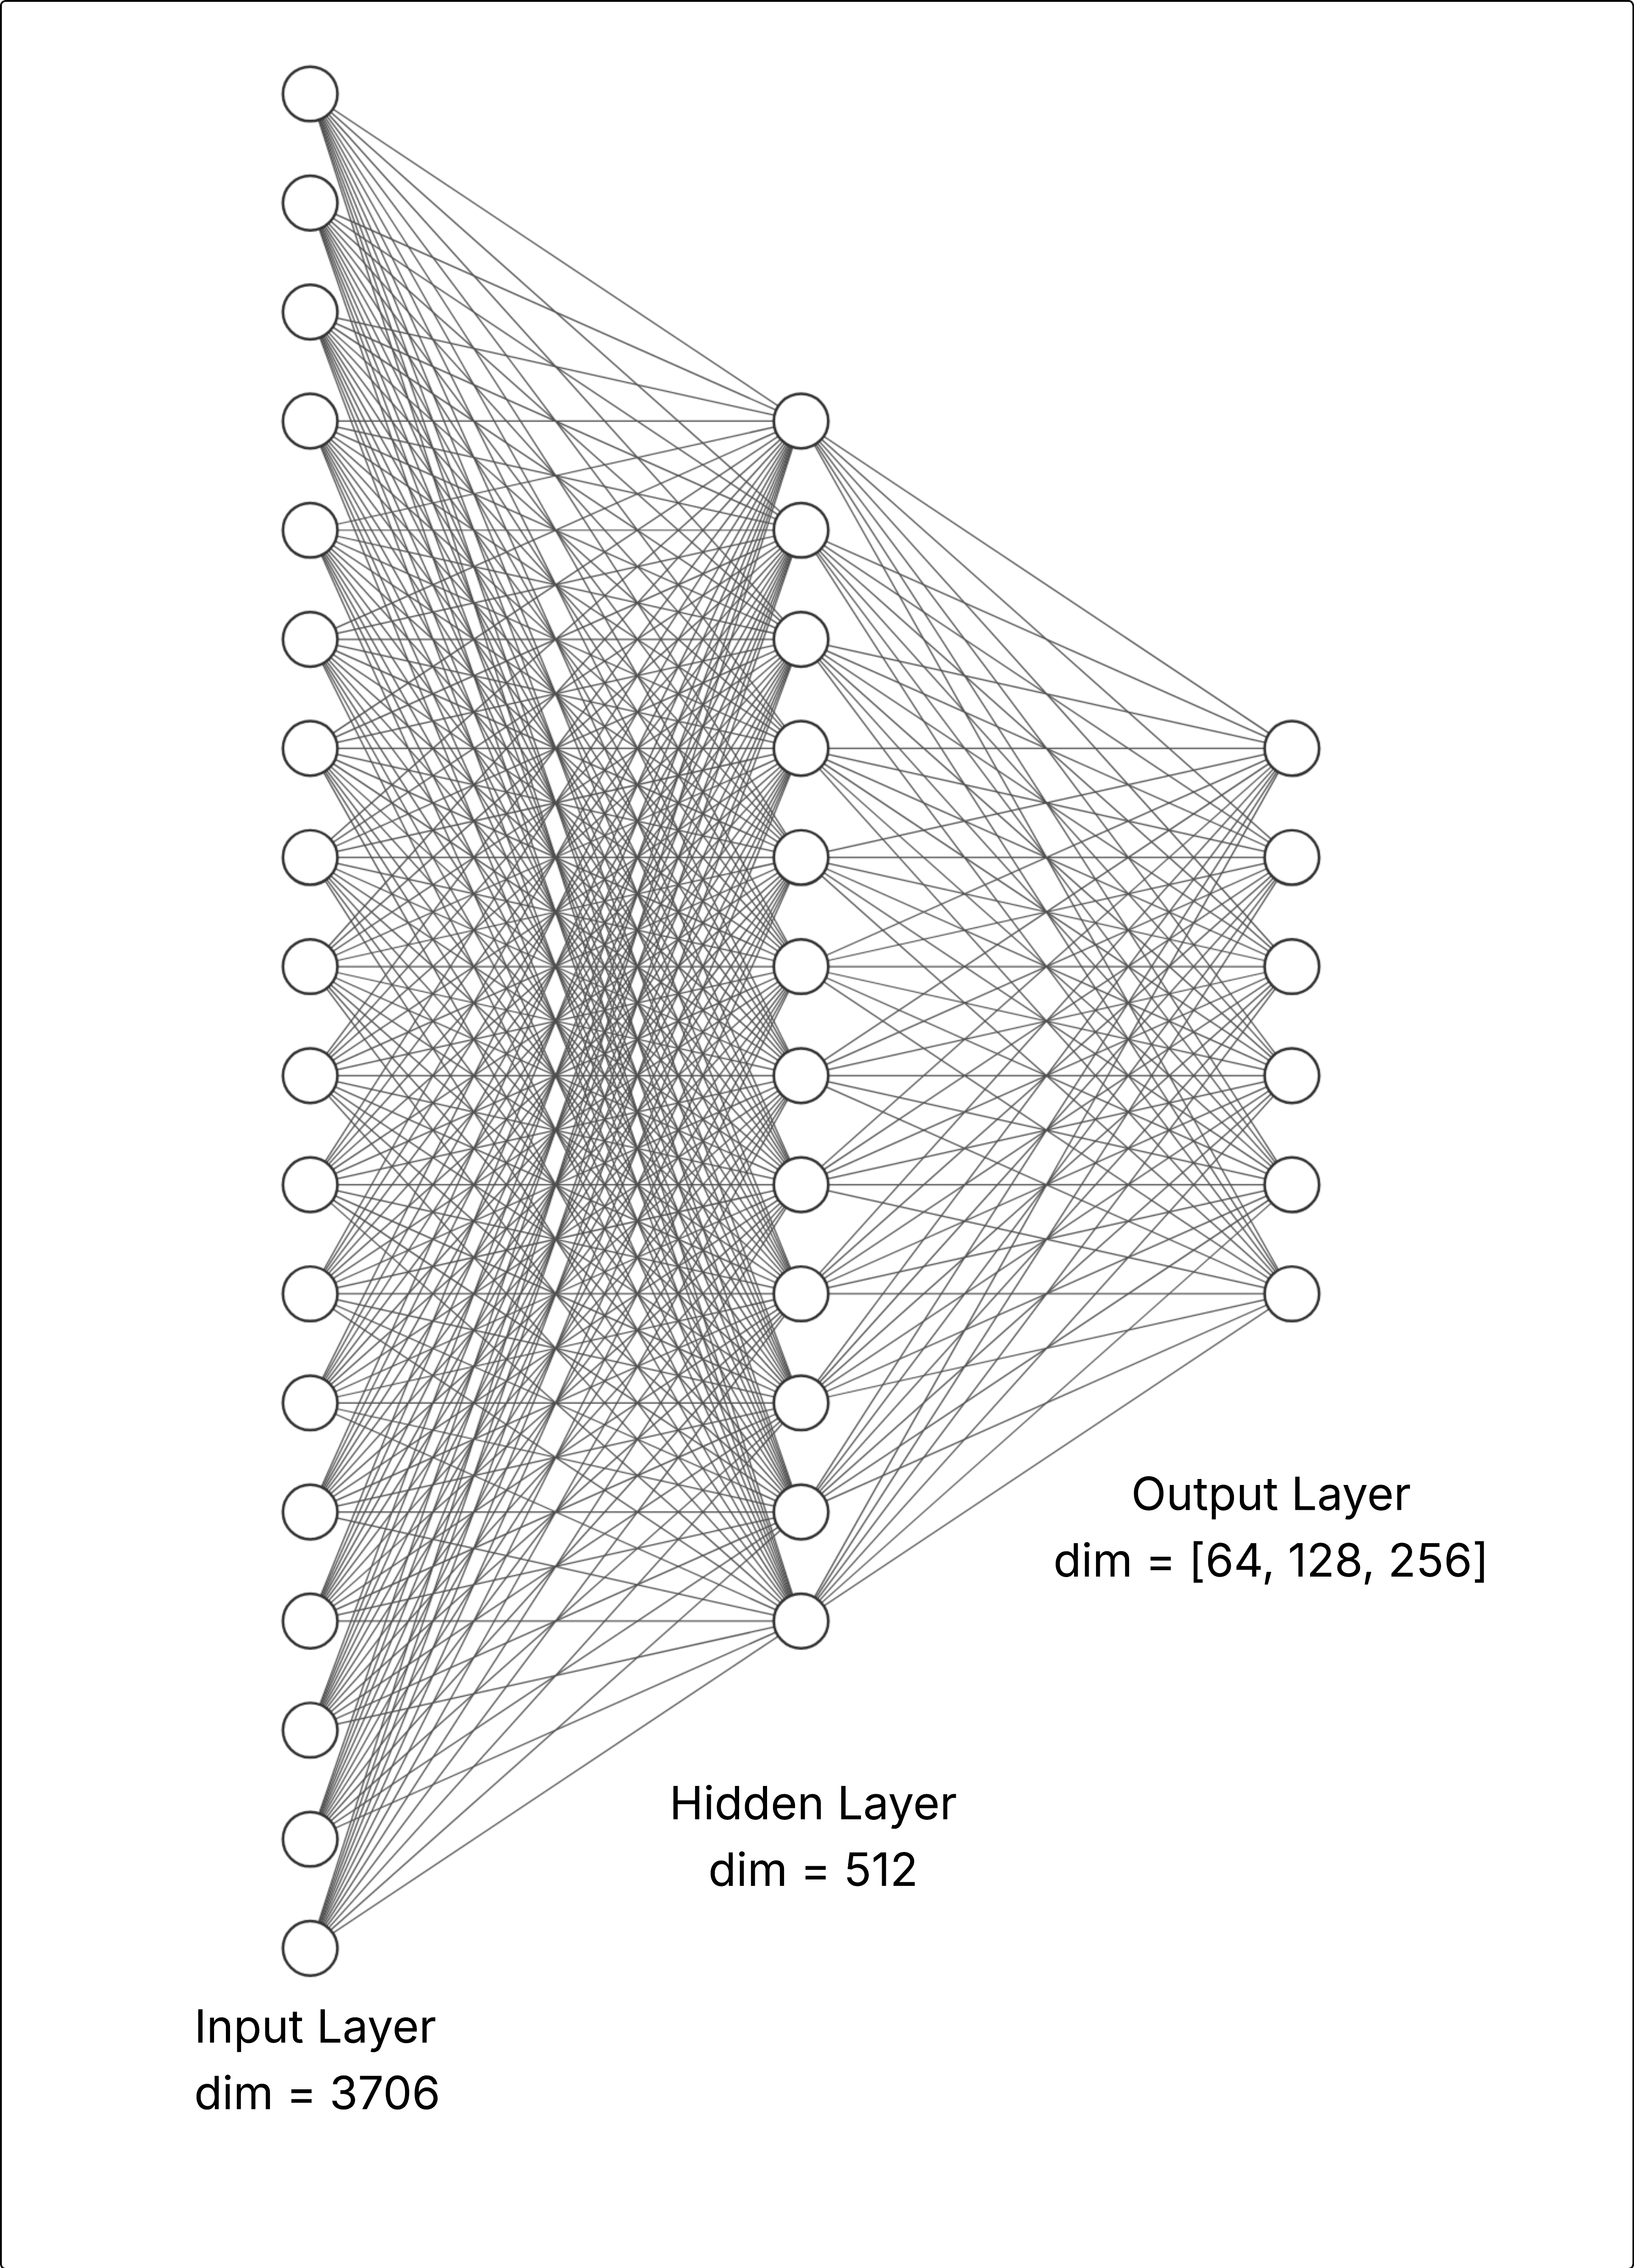
\includegraphics[width=0.5\textwidth]{figures/mlp_architecture.png}
    \caption{MLP architecture for user embedding generation (input: 3706, hidden: 512, output: embedding size).}
    \label{fig-mlp_architecture}
\end{figure}

After the embeddings are learned, clustering is performed separately in
each embedding space. The four clustering methods considered are
K-means, probabilistic distance clustering (PD), reduced K-means (RKM),
and factorial probabilistic distance clustering (FPDC). The experimental
design applies each method to each embedding dimension in order to
compare clustering behavior across both representation size and
clustering algorithm.

Clustering is not performed directly on the raw sparse rating matrix.
Instead, the embedding model transforms sparse user--item behavior into
a lower-dimensional representation on which clustering is applied.

\subsection{Clustering Implementation in
R}\label{clustering-implementation-in-r}

We ran all four clustering analyses in R. Before clustering, we
standardized every embedding matrix so that each embedding coordinate
contributed on a comparable scale to Euclidean-distance calculations. We
cached every fitted model and tuning result to \texttt{.rds} files so
that we could reproduce tables and figures without rerunning the full
pipeline during rendering. As described in the Dataset section, all
clustering experiments were conducted on the MovieLens 1M embeddings.

We implemented K-means (Everitt et al. 2011) with the \texttt{kmeans()}
function from the base \texttt{stats} package. During tuning, we
compared the Hartigan--Wong, Lloyd, and MacQueen algorithmic variants
with 10 random starts and a maximum of 100 iterations. The three
variants led to the same substantive tuning conclusion: in every
embedding dimension, they attained their best silhouette and
Calinski-Harabasz (CH) values at 2 clusters, and the metric differences
between variants were small. We selected MacQueen as the final reported
K-means implementation because it provided the strongest overall
runtime--quality tradeoff and the cleanest fitting behavior across
embeddings. For K-means tuning, we evaluated cluster counts from 2
through 20 so that we could inspect the full within-cluster sum of
squares curve. For the cross-method comparison, we used the saved
MacQueen models over cluster counts 2 through 8.

We implemented RKM (De Soete and Carroll 1994) with \texttt{cluspca()}
from the \texttt{clustrd} package, using \texttt{method\ =\ "RKM"} and
\texttt{rotation\ =\ "varimax"}. We jointly tuned the number of clusters
\((k \in \{2, \ldots, 10\})\) and the number of retained factors
\((q \in \{2, \ldots, 6\})\). RKM estimates both a partition and a
lower-dimensional subspace, so each additional retained factor increases
computational cost. We selected the final RKM model in each embedding
with average silhouette width as the primary criterion and the CH index
as the secondary criterion.

We implemented PD (Ben-Israel and Iyigun 2008) with \texttt{PDC()} from
the \texttt{FPDclustering} package (Tortora et al. 2024). For each
embedding dimension, we evaluated candidate cluster counts from 2
through 10. PD does not estimate an additional reduced subspace, so it
remained computationally inexpensive relative to RKM and FPDC and
therefore supported a broader cluster-count search. We selected the
final PD model in each embedding with probability silhouette as the
primary criterion, ordinary silhouette as the secondary criterion, and
the CH index as the tertiary criterion.

FPDC (Tortora et al. 2016) was implemented using \texttt{FPDC()} from
the \texttt{FPDclustering} package (Tortora et al. 2024). Models were
fit over the grid \(k \in \{2, \ldots, 8\}\) and
\(q \in \{2, \ldots, 5\}\), using 20 internal iterations and tuning
parameters \(\nu = 6\) and \(\nu = 10\). Preliminary runs with
\(\nu = 2\) produced highly inconsistent solutions and were therefore
excluded from the final reported analysis. We selected the best FPDC
model per embedding using probability silhouette as the primary
criterion, ordinary silhouette as the secondary criterion, and the CH
index as the tertiary criterion.

\section{Test Setup and Evaluation}\label{sec-evaluation-framework}

Because the analysis has no ground-truth labels, we evaluated the
clustering results with internal validation metrics, bootstrap
stability, partition agreement, empirical runtime, and interpretability
rather than external criteria.

\subsection{Internal Validation
Metrics}\label{internal-validation-metrics}

We used \textbf{average silhouette} (Kaufman and Rousseeuw 1990) width
as the main hard-clustering diagnostic for K-means and RKM. Silhouette
width measures how much closer each user lies to its assigned cluster
than to the nearest competing cluster, so larger values indicate
better-separated and more coherent clusters. We used the
\textbf{Calinski-Harabasz (CH)} index as a second hard-clustering
diagnostic because it rewards high between-cluster dispersion and low
within-cluster dispersion.

For PD and FPDC, we also computed probability silhouette with
\texttt{Silh()} from the \texttt{FPDclustering} package (Tortora et al.
2024). Probability silhouette respects soft memberships and therefore
aligns more closely with the probabilistic objective than ordinary
silhouette alone. We still report ordinary silhouette and the CH index
for those methods so that we can compare the soft-clustering methods
with the hard-clustering methods on a common scale.

For K-means, we also reported total within-cluster sum of squares
because it directly reflects the K-means objective. We used the
within-cluster sum of squares curve as the primary K-means tuning
diagnostic and extracted the elbow from the saved fitted models. Because
within-cluster sum of squares decreases monotonically as the number of
clusters increases, we interpreted the elbow as a method-specific
structural diagnostic rather than as a measure of cluster separation.

We selected each method with a \textbf{method-specific hierarchy} of
criteria shown in Table \ref{tbl-tuning-summary}.

\begin{table}

\caption{\label{tbl-tuning-summary}Tuning ranges and model-selection rules for each clustering method.}

\centering{

[htbp]
\centering
\small


\resizebox{\textwidth}{!}{
\begin{tabular}{llllll}
\toprule
Method & Cluster-counts & Retained-factors & $1^{st}$ criterion & $2^{nd}$ criterion & $3^{rd}$ criterion \\
\midrule
KM & 2--20 & -- &  WSS elbow diagnostic & Avg. silhouette width & CH \\
RKM & 2--10 & 2--6 & Avg. silhouette width for all (k,q) combinations & CH & Bootstrap stability \\
PD & 2--5 & -- & Probability silhouette & Avg. silhouette width & CH \\
FPDC & 2--8 & 2--5 & Probability silhouette for all (k,q, $\nu$) combinations &  Silhouette width & CH index \\
\bottomrule
\end{tabular}
}

}

\end{table}%

\subsection{Stability}\label{stability}

We assessed bootstrap stability with 15 bootstrap replicates for each
combination of method, embedding dimension, and cluster count (Everitt
et al. 2011). In each replicate, we sampled 30\% of users with
replacement, refit the clustering model on the bootstrap sample, and
compared the resulting partition with the full-data reference partition
by \textbf{adjusted Rand index (ARI)} (Kaufman and Rousseeuw 1990). ARI
ranges from 0 for chance-level agreement to 1 for perfect agreement, so
larger values indicate more reproducible solutions. For PD and FPDC, we
converted soft memberships to hard labels by assigning each user to the
cluster with the highest membership probability before computing ARI.

We also compared the final partitions across methods with pairwise
adjusted Rand indices computed within matched embedding dimensions and
matched cluster counts. This comparison tells us whether different
methods recover the same underlying structure or fundamentally different
partitions.

\subsection{Runtime and Computational
Cost}\label{runtime-and-computational-cost}

We recorded wall-clock runtime for every cached model fit and used
runtime as an empirical measure of computational complexity. K-means and
PD mainly scale with repeated distance calculations between users and
cluster centers, so they remain comparatively fast. RKM adds the cost of
estimating and rotating a lower-dimensional subspace. FPDC adds both
subspace estimation and iterative soft-membership updates, and it also
tunes \(\nu\). We therefore interpreted runtime jointly with fit
quality: a more complex method should deliver a clear gain in clustering
quality if it is going to justify higher computational cost.

\subsection{Implementation Summary}\label{implementation-summary}

Table \ref{tbl-tuning-summary} summarizes the parameter search grids and
model-selection rules for each clustering method. The methods differ in
how many parameters must be specified: K-means requires only the number
of clusters \(k\), which allows a broad search range and a full WSS
elbow diagnostic. RKM requires both \(k\) and the number of retained
factors \(q\), so the search grid grows more quickly. FPDC additionally
requires \(\nu\), which further expands the parameter space and
motivated a more compact retained-factor range relative to RKM. The
Tucker-factor (See Appendix Figure \ref{fig-tucker-factor}) diagnostic
increased smoothly with the number of retained factors and did not show
a sharp elbow, which confirmed that large retained-factor values offered
only incremental gains.

All methods were applied to standardized embedding matrices of
dimensions 64, 128, and 256. For K-means, WSS elbow plots were used as a
method-specific tuning diagnostic, and the final value of \(k\) was
determined using silhouette width, the CH index, and bootstrap stability
when the elbow was weak or ambiguous. For RKM, \(k\) and the reduced
dimension \(q\) were selected jointly over a two-dimensional grid using
silhouette as the primary criterion and CH as a secondary check. For the
probabilistic methods, model selection emphasized probability silhouette
because PD and FPDC produce soft cluster memberships. Accordingly, PD
models were selected over \(k\) using probability silhouette as the
primary criterion, with ordinary silhouette and CH used as supporting
diagnostics, while FPDC models were selected over \((k, q, \nu)\) using
the same hierarchy. Intermediate results were cached to R Data
Serialization or \texttt{.rds} files to support reproducibility without
rerunning the full pipeline during rendering.

\section{Results}\label{sec-results}

This section compares clustering performance across embedding dimensions
and methods using the pre-specified method-specific tuning criteria,
with average silhouette width, the CH index, runtime, and bootstrap
stability used to interpret the selected solutions.

\begin{table}

\caption{\label{tbl-best-models}Best clustering result for each method and embedding dimension under the pre-specified method-specific selection criteria. Runtime is reported in seconds.}

\centering{

[htbp]
\centering
\small


\begin{tabular}{llrrrrrrr}
\toprule
Method & Embedding & Clusters & Factors & $\nu$ & Runtime & Silhouette & CH index & Prob.\ silh. \\
\midrule
K-means & 64  & 4 & --- & --- & 7.35  & -0.011 & 96.96  & --- \\
PD & 64  & 2 & --- & --- & 0.29  & 0.003  & 10.14  & 0.093 \\
RKM & 64  & 2 & 2 & --- & 278.90 & 0.235 & 132.29 & --- \\
FPDC & 64  & 2 & 4 & 6  & 241.74 & 0.012 & 70.55  & 0.143 \\
K-means & 128 & 4 & --- & --- & 12.72 & -0.010 & 91.21  & --- \\
PD & 128 & 2 & --- & --- & 0.18  & 0.000  & 0.92   & 0.068 \\
RKM & 128 & 2 & 4 & --- & 184.10 & 0.331 & 139.52 & --- \\
FPDC & 128 & 4 & 2 & 6  & 188.16 & -0.115 & 56.43 & 0.136 \\
K-means & 256 & 4 & --- & --- & 23.45 & 0.026  & 74.77  & --- \\
PD & 256 & 2 & --- & --- & 0.26  & 0.000  & 1.07   & 0.062 \\
RKM & 256 & 2 & 5 & --- & 257.64 & 0.290 & 111.25 & --- \\
FPDC & 256 & 6 & 3 & 10 & 70.74 & -0.209 & 33.92 & 0.148 \\
\bottomrule
\end{tabular}

}

\end{table}%

Table \ref{tbl-best-models} reports the final selected model for each
method and embedding dimension under the pre-specified method-specific
tuning rules. Under these rules, RKM produced the strongest overall hard
partitions. The best overall solution used the 128-dimensional
embeddings, 2 clusters, and 4 retained factors, and it achieved an
average silhouette width of 0.331 and a CH index of 139.52. The
256-dimensional RKM model followed with 2 clusters and 5 retained
factors, silhouette 0.290, and CH index 111.25. The 64-dimensional RKM
model selected 2 clusters and 2 retained factors and achieved silhouette
0.235 and CH index 132.29.

K-means behaved differently under the revised selection rules because we
prioritized the within-cluster sum of squares elbow diagnostic. The
elbow diagnostic selected 4 clusters in all three embedding dimensions.
Those selected K-means solutions achieved silhouettes of -0.011, -0.010,
and 0.026 in the 64-, 128-, and 256-dimensional embeddings,
respectively. These values are much lower than the corresponding
two-cluster silhouette values, which means the elbow-based K-means rule
favored a more complex partition than the silhouette-based rule would
have favored. This contrast is important: under the revised
method-specific criteria, K-means no longer provides the strongest
selected solution.

Figure \ref{fig-best-silhouette-by-method} summarizes the best selected
silhouette value for each method and embedding dimension. The figure
shows that the 128-dimensional embeddings still provide the clearest
overall structure, but the selected winner now depends on the tuning
rule attached to each method. RKM dominates K-means under the revised
criteria because RKM directly selects its best model by silhouette,
while K-means now selects its model by the elbow diagnostic. The
64-dimensional embeddings appear too compressed to capture the full
geometry of user preferences, while the 256-dimensional embeddings
retain useful structure but do not surpass the 128-dimensional
representations.

\begin{figure}[htbp]
    \centering
    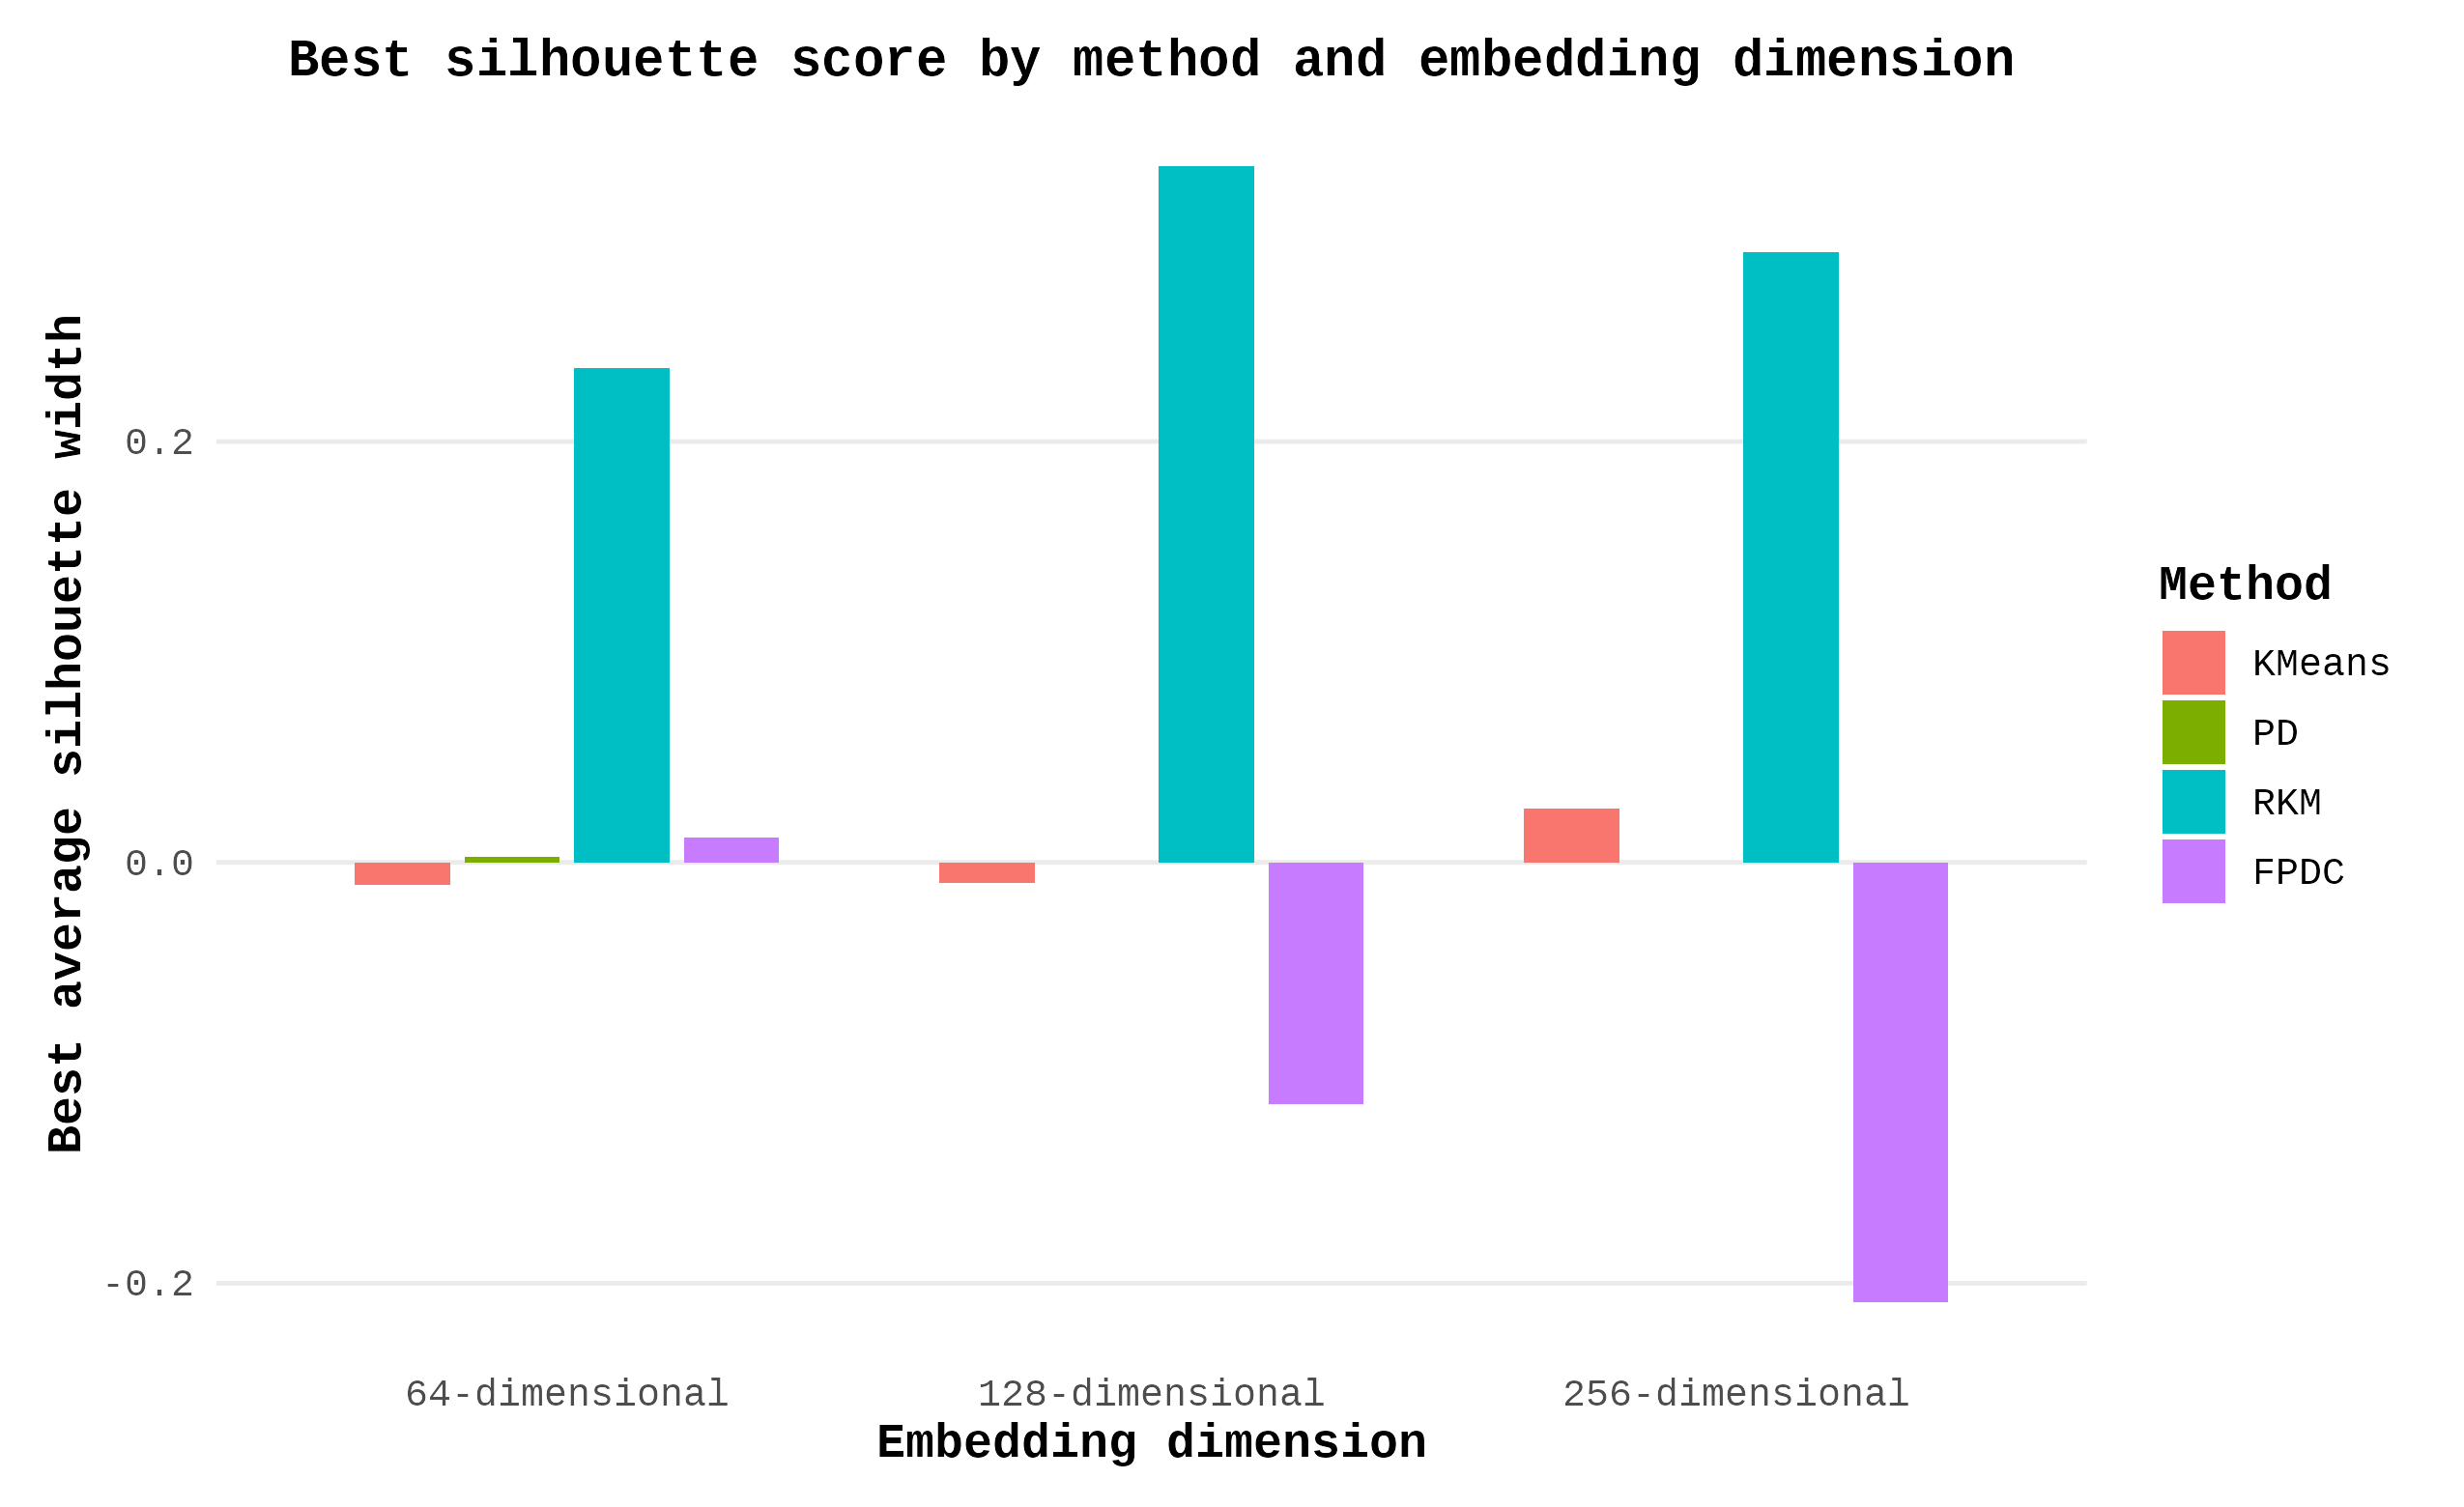
\includegraphics[width=0.8\textwidth]{figures/figure3_best_silhouette_by_method_embedding.png}
    \caption{Best selected silhouette value by method and embedding dimension under the pre-specified method-specific tuning rules.}
    \label{fig-best-silhouette-by-method}
\end{figure}

Figure \ref{fig-runtime-tradeoff} compares runtime and clustering
quality for the final selected models. PD ran fastest in every embedding
dimension, with runtimes between 0.18 and 0.29 seconds, but it produced
ordinary silhouette values at or near zero. K-means ran much faster than
RKM and FPDC, with selected-model runtimes of 7.35, 12.72, and 23.45
seconds, but the elbow-selected K-means models did not produce strong
hard partitions. RKM required 184.10 to 278.90 seconds because it
jointly estimated a partition and a lower-dimensional subspace. FPDC
required 70.74 to 241.74 seconds for the selected models and still
produced weak or negative ordinary silhouettes. In practical terms, RKM
delivered the best hard-clustering quality, but it did so at
substantially higher computational cost than K-means or PD.

\begin{figure}[htbp]
    \centering
    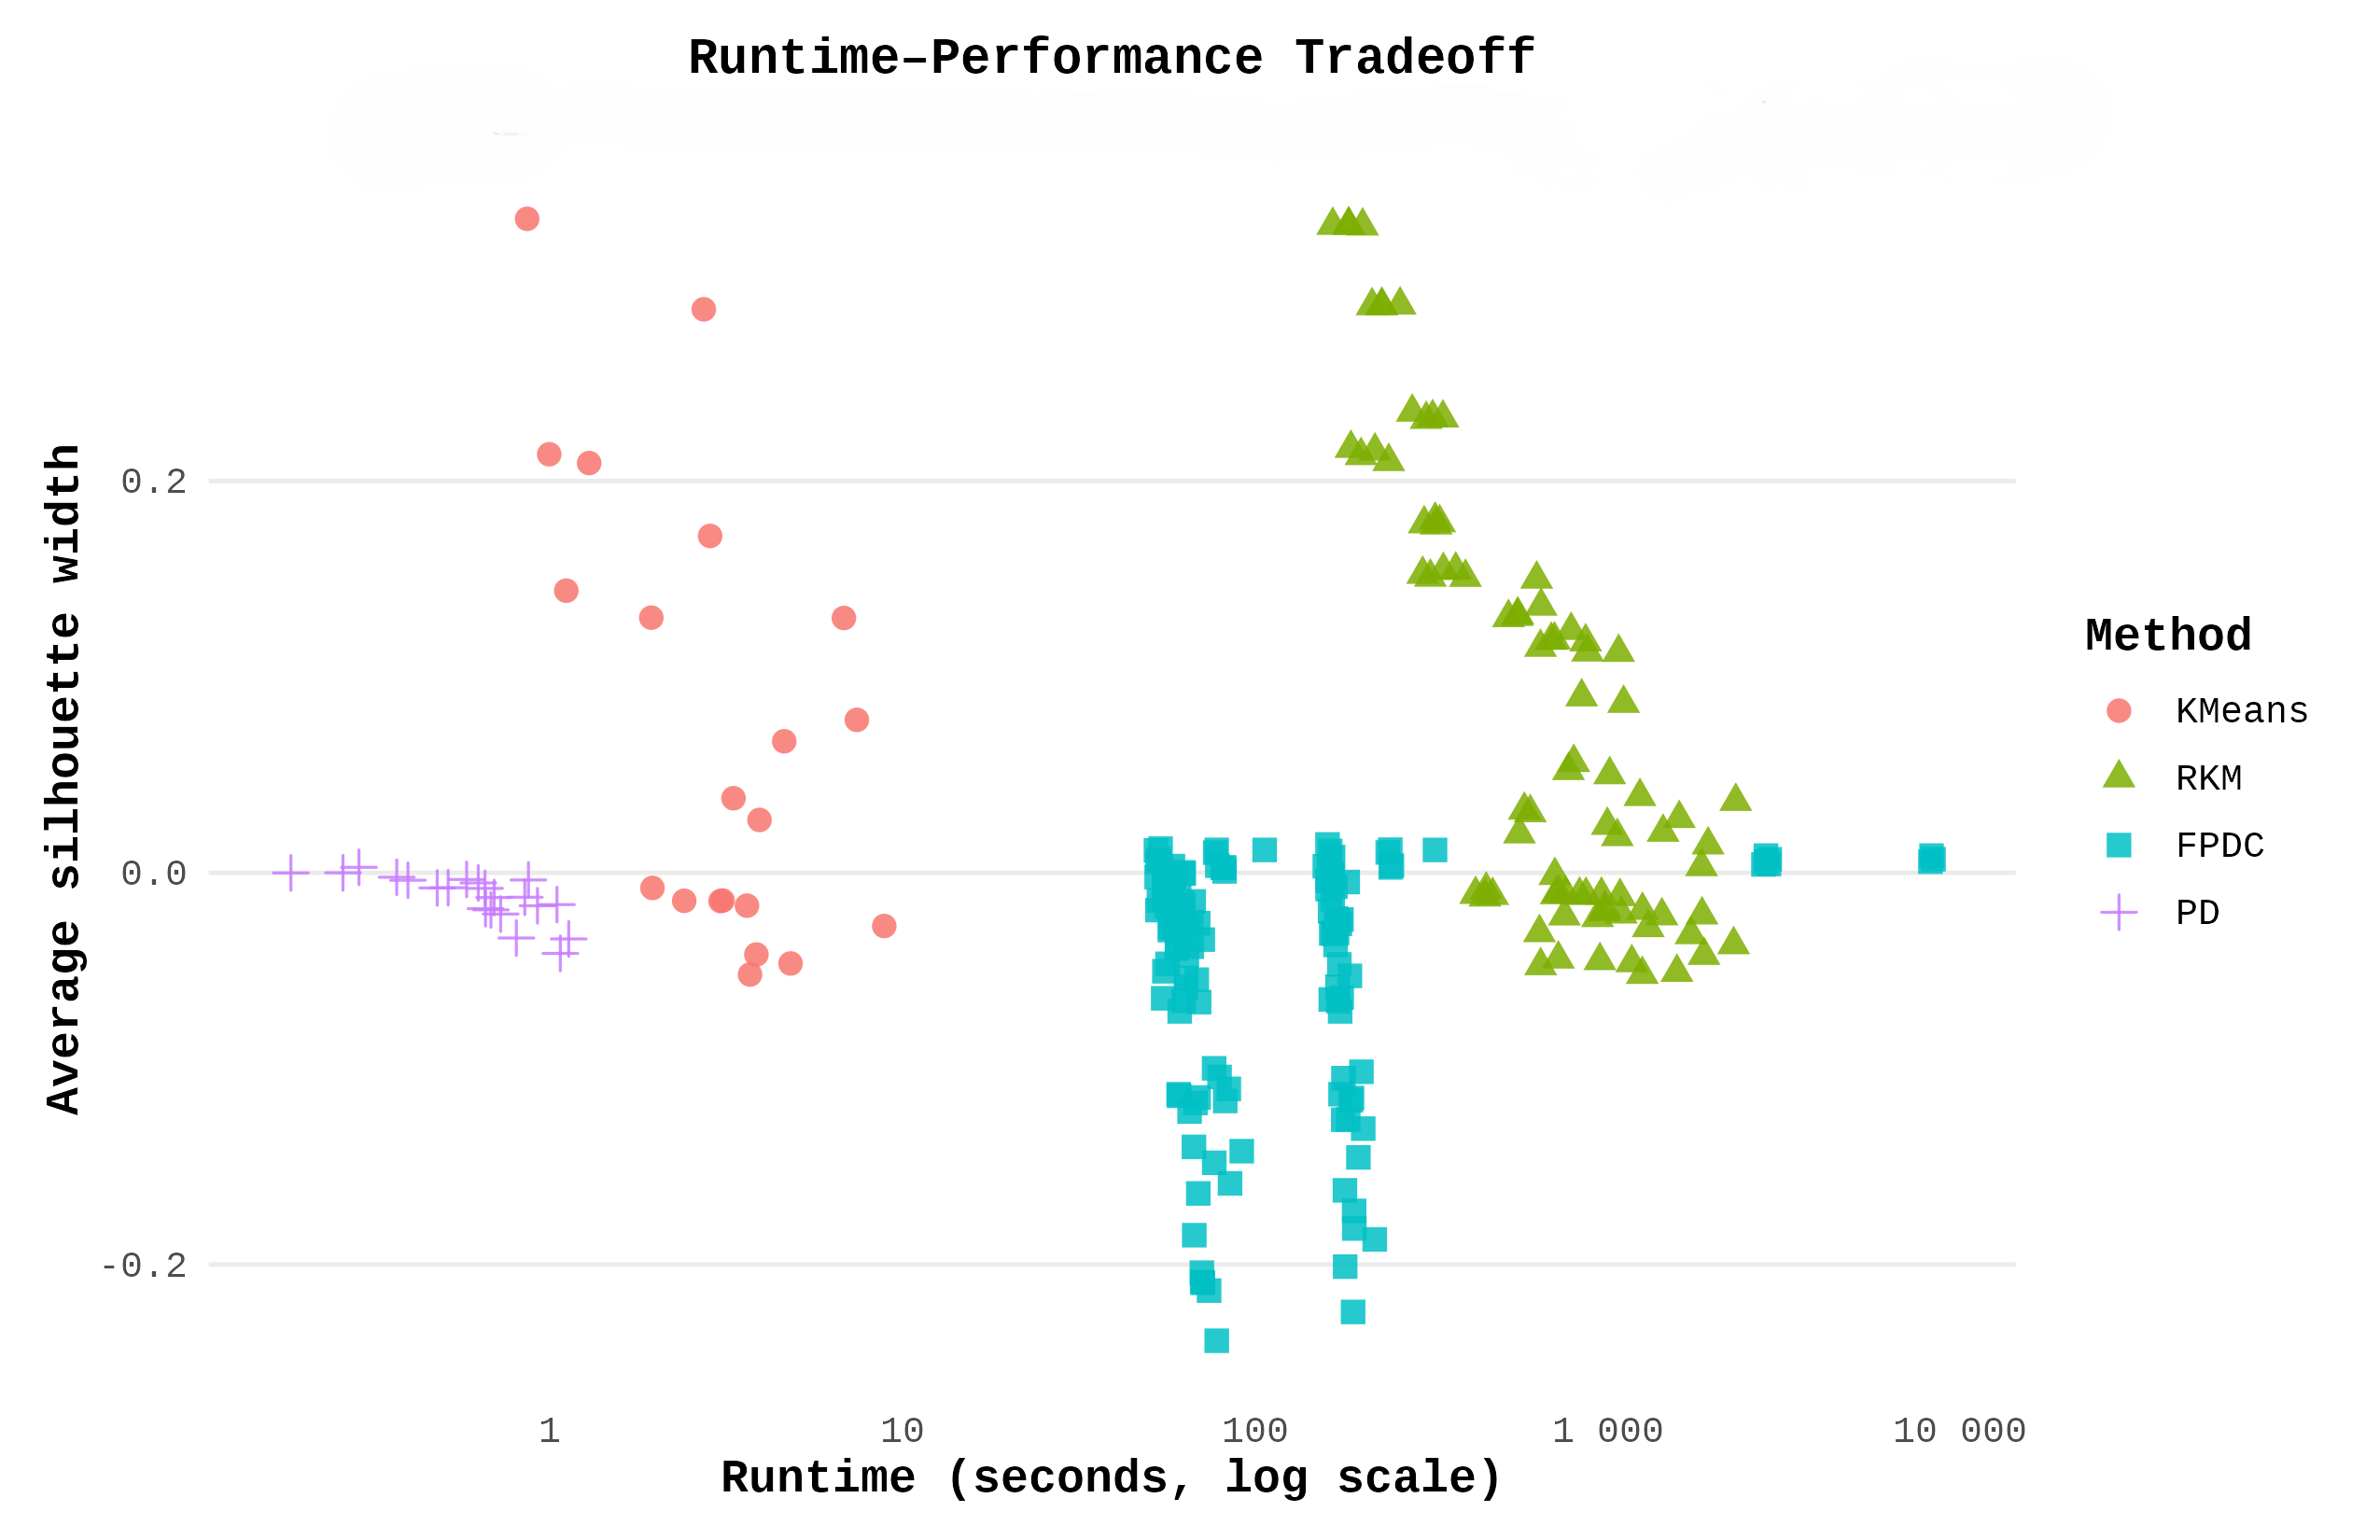
\includegraphics[width=0.8\textwidth]{figures/figure3_runtime_vs_silhouette.png}
    \caption{Runtime and clustering quality for the final selected models.}
    \label{fig-runtime-tradeoff}
\end{figure}

Figure \ref{fig-runtime-tradeoff} therefore serves as an empirical
complexity summary: methods with larger tuning grids and more expensive
updates move to the right, and only RKM shows a clear quality gain that
partly justifies that extra cost.

PD selected 2 clusters in all three embedding dimensions because
probability silhouette favored that solution throughout the PD grid.
Even so, the selected PD models remained weak: the ordinary silhouette
values were 0.003, 0.000, and 0.000 in the 64-, 128-, and
256-dimensional embeddings, and the probability silhouettes were only
0.093, 0.068, and 0.062. These results indicate that PD did not recover
a strong hard partition in the learned user embeddings.

FPDC performed better than PD on the probability-silhouette criterion,
but it still did not recover competitive hard partitions. In the
64-dimensional embedding, FPDC selected 2 clusters, 4 retained factors,
and \(\nu=6\), with probability silhouette 0.143 and ordinary silhouette
0.012. In the 128-dimensional embedding, FPDC selected 4 clusters, 2
retained factors, and \(\nu=6\), with probability silhouette 0.136 and
ordinary silhouette -0.115. In the 256-dimensional embedding, FPDC
selected 6 clusters, 3 retained factors, and \(\nu=10\), with
probability silhouette 0.148 and ordinary silhouette -0.209. FPDC
therefore improved the soft-membership diagnostic relative to PD, but
that improvement did not translate into a strong hard partition.

Figure \ref{fig-ari-method-pairs} compares the final partitions across
methods with average ARI. K-means and RKM still show by far the
strongest agreement, with average ARI 0.586. This result indicates that
both methods recover a closely related underlying structure, even though
the revised K-means selection rule now reports 4 clusters. Method pairs
involving PD or FPDC show much weaker agreement. FPDC versus RKM
averages 0.061, FPDC versus K-means averages 0.060, FPDC versus PD
averages 0.007, and both K-means versus PD and RKM versus PD average
0.001. These low values indicate that the probabilistic methods
recovered fundamentally different and much less stable partitions.

\begin{figure}[htbp]
    \centering
    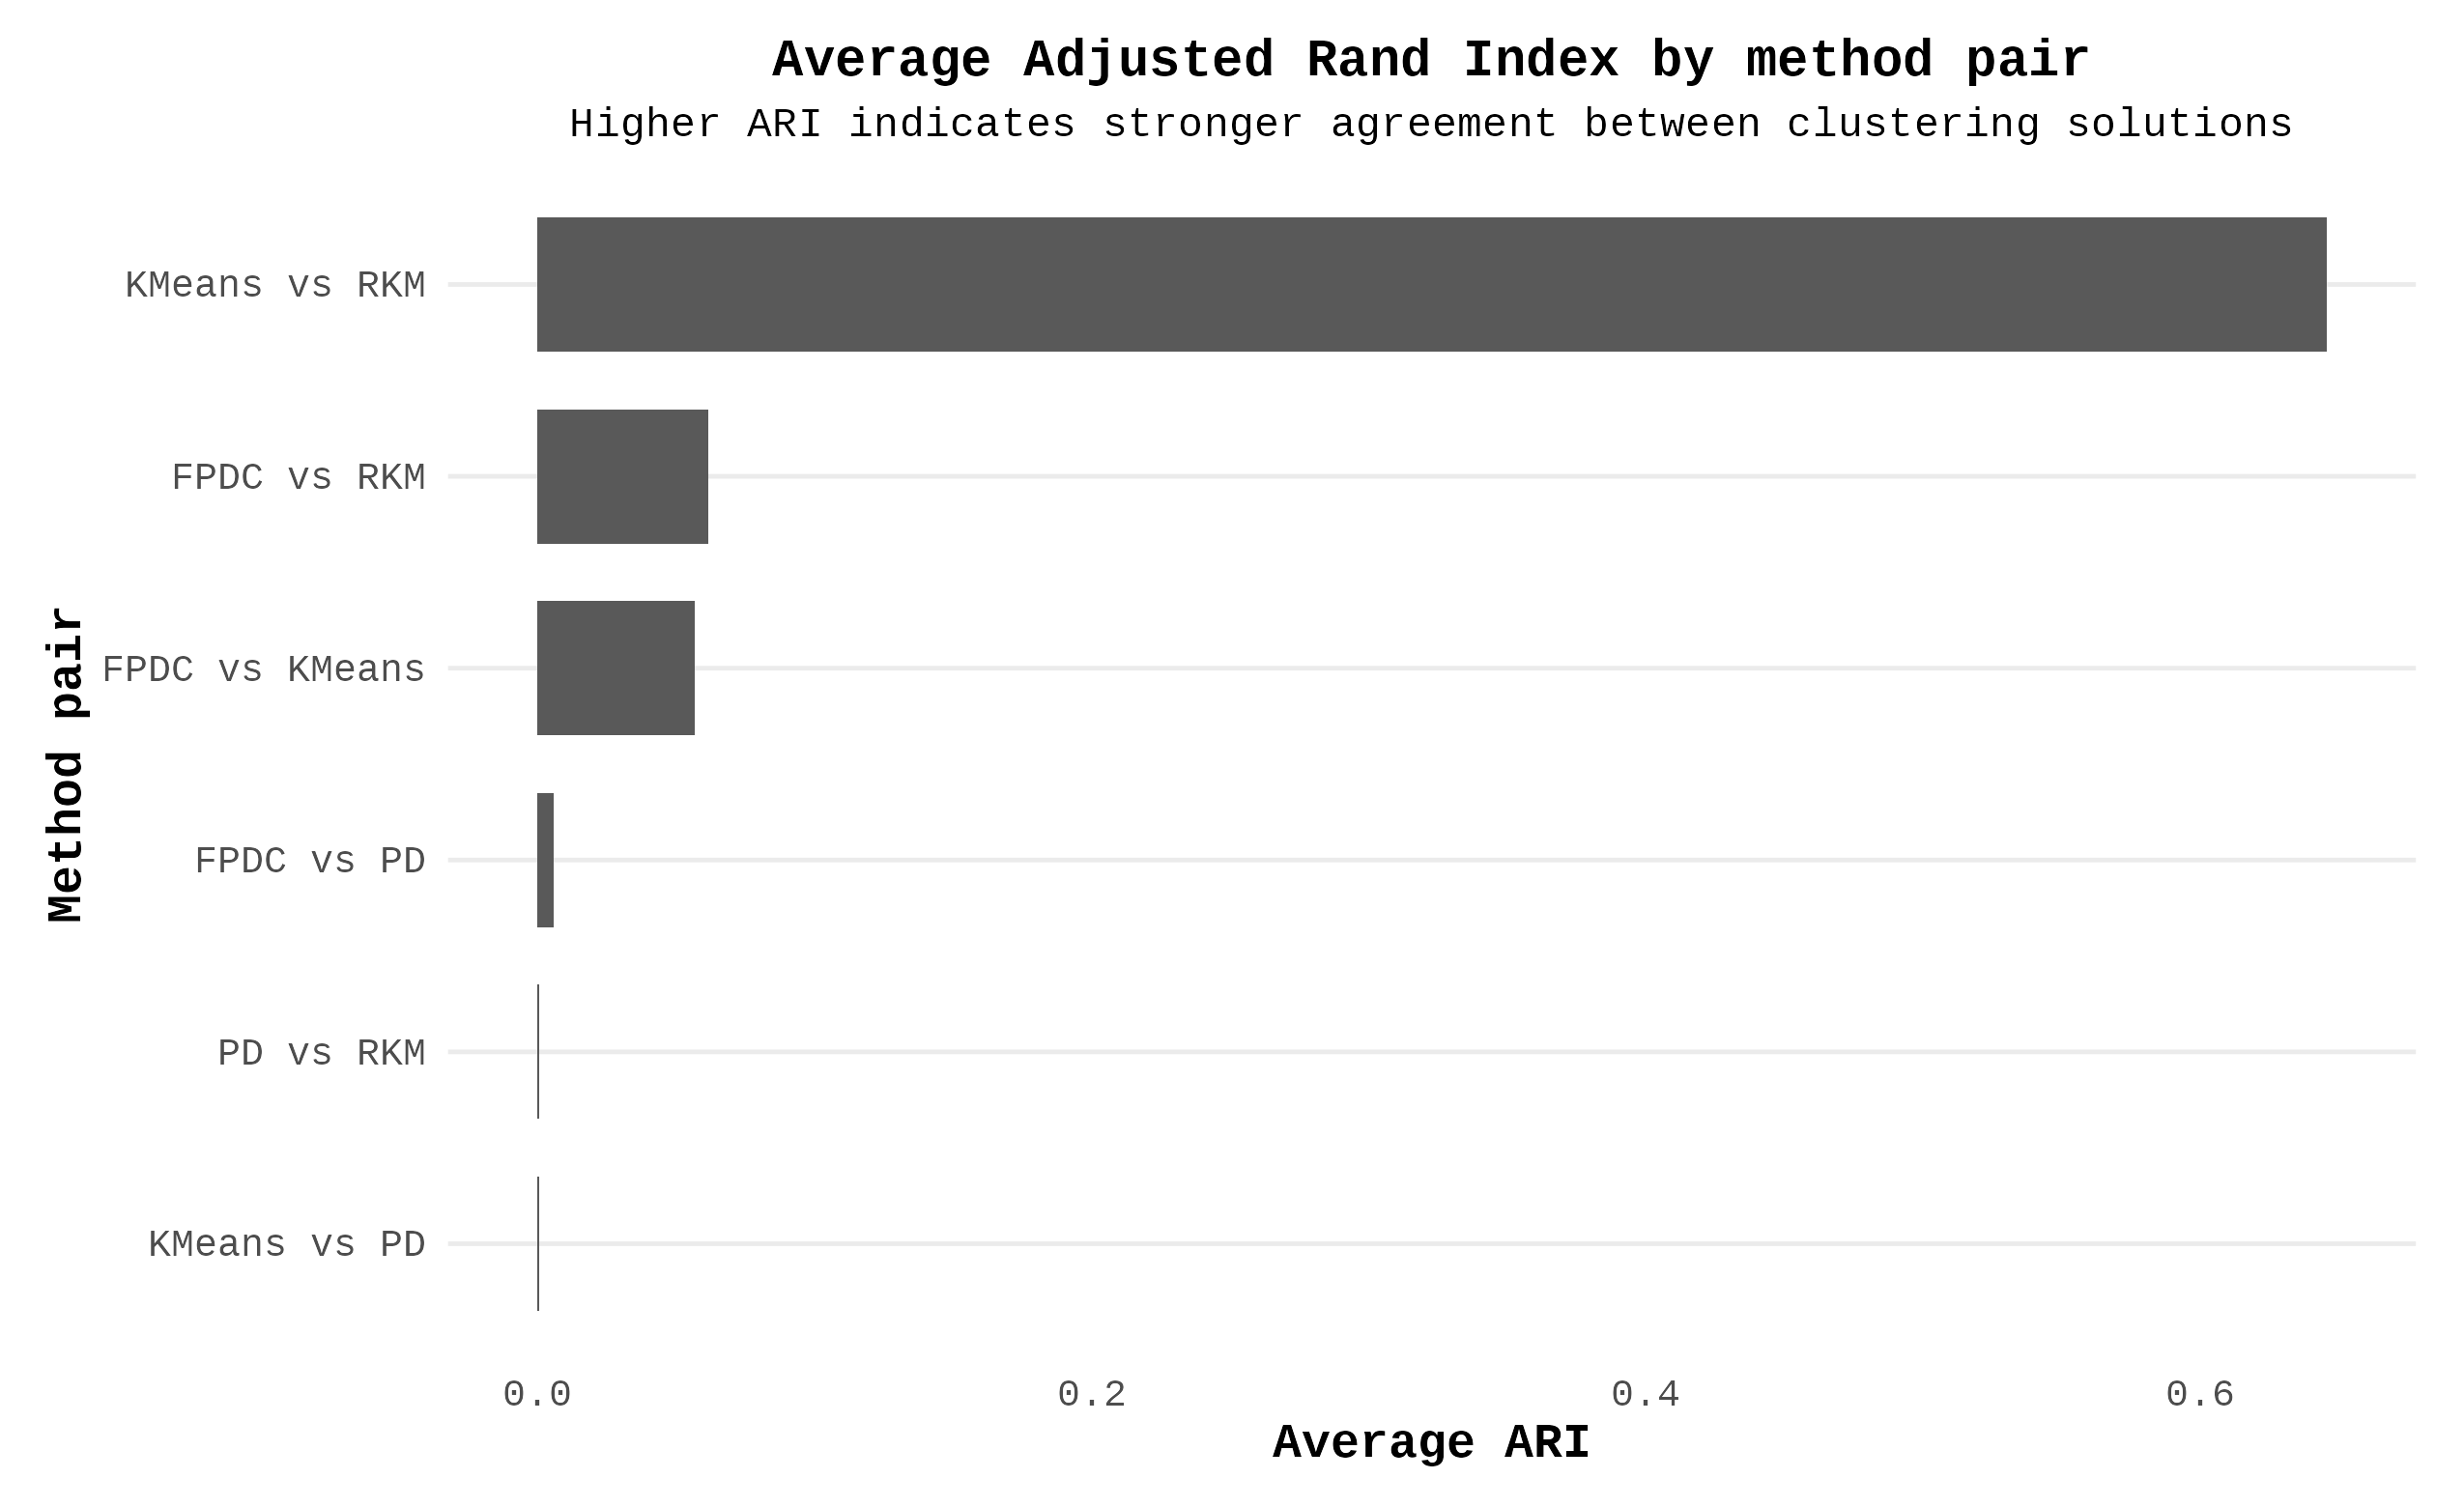
\includegraphics[width=0.8\textwidth]{figures/figure4_average_ari_by_method_pair.png}
    \caption{Average ARI by method pair. Higher values indicate stronger agreement between partitions recovered by different clustering methods.}
    \label{fig-ari-method-pairs}
\end{figure}

\subsection{Stability Analysis}\label{sec-stability}

K-means and RKM are the only methods that produce clearly reproducible
partitions. Across embedding dimensions, both methods show their highest
mean bootstrap ARI at 2 clusters, with stability weakening as the number
of clusters increases. This pattern is especially consistent for RKM and
supports the final two-cluster RKM solutions. For K-means, the stability
results favor 2 clusters, which contrasts with the elbow-based selection
of 4 clusters and highlights the sensitivity of K-means to the chosen
tuning criterion.

PD and FPDC do not exhibit comparable reproducibility. PD maintains mean
bootstrap ARI values near zero across almost all settings, which
indicates that its partitions are not stable under resampling. FPDC
shows slightly positive stability in some settings, but the values
remain low and inconsistent. Occasional local increases around 3
clusters are not large enough to provide evidence of a reliable
partition.

Overall, the stability analysis reinforces the earlier results: only RKM
and K-means recover a reproducible structure for two clusters, while PD
and FPDC yield unstable partitions. Bootstrap stability plots of mean
ARI across clustering method, embedding dimension, and number of
clusters are provided in Appendix Section~\ref{sec-appendix} Figure
\ref{fig-stability}.

\subsection{\texorpdfstring{FPDC Sensitivity to the Tuning Parameter
\(\nu\)}{FPDC Sensitivity to the Tuning Parameter \textbackslash nu}}\label{sec-fpdc-nu}

We evaluated FPDC at \(\nu = 2\), \(\nu = 6\), and \(\nu = 10\). Pilot
runs with \(\nu = 2\) produced highly inconsistent solutions and did not
improve either probability silhouette or ordinary silhouette beyond
chance-like behavior, so we excluded \(\nu = 2\) from the final
sensitivity summary. Table Table~\ref{tbl-fpdc-nu-sensitivity} reports
the best FPDC result within each retained \(\nu\) value for each
embedding dimension.

The 64-dimensional embedding changed very little between \(\nu = 6\) and
\(\nu = 10\). Both settings selected 2 clusters and 4 retained factors,
and both produced probability silhouette 0.143 with ordinary silhouette
about 0.012. The 128-dimensional embedding also changed very little
between \(\nu = 6\) and \(\nu = 10\). Both settings selected 4 clusters
and 2 retained factors, and both produced probability silhouette near
0.136 with negative ordinary silhouette. The 256-dimensional embedding
showed the clearest difference. There, \(\nu = 6\) selected 3 clusters
and 2 retained factors, with probability silhouette 0.146, ordinary
silhouette -0.056, and Calinski-Harabasz index 63.41. By contrast,
\(\nu = 10\) selected 6 clusters and 3 retained factors, with slightly
higher probability silhouette 0.148 but much worse ordinary silhouette
-0.209 and a lower Calinski-Harabasz index of 33.92. In this dataset,
increasing \(\nu\) could improve FPDC's soft-membership objective while
degrading the corresponding hard partition.

\section{Conclusion and Future
Work}\label{sec-conclusion-and-future-work}

This study evaluated clustering structure in user embeddings learned
from the MovieLens 1M dataset across multiple embedding dimensions and
clustering methods. Overall, the results provide only modest evidence of
clustering structure in the learned representations. None of the methods
produced uniformly strong results across evaluation criteria, and
several selected solutions exhibited weak separation or poor
reproducibility.

Among the methods considered, RKM produced the strongest and most
consistent hard-clustering results. Its best solution, obtained in the
128-dimensional embedding space with 2 clusters and 4 retained factors,
achieved the highest silhouette and strong CH values. K-means produced
closely related partitions, as shown by high agreement with RKM, but its
conclusions depended strongly on the tuning rule. In particular, the
within-cluster sum of squares elbow diagnostic favored 4-cluster
solutions with substantially weaker separation than the corresponding
2-cluster solutions. This sensitivity weakens the interpretability of
K-means as a standalone method in this setting.

The probabilistic methods (PD and FPDC) provided less convincing
results. PD consistently selected 2 clusters but produced near-zero
silhouette values and showed little bootstrap stability. FPDC improved
the probability-silhouette criterion relative to PD, but this
improvement did not translate into meaningful hard partitions. FPDC
solutions often exhibited negative silhouette values, low agreement with
K-means and RKM, and higher computational cost. Sensitivity to the
tuning parameter \(\nu\) further complicated interpretation, as
improvements in the soft objective could coincide with degradation in
hard-clustering quality.

These results suggest that the learned user embeddings contain limited
and weakly separated cluster structure. The consistent selection of
two-cluster solutions by the strongest-performing methods indicates that
the dominant signal in the embedding space may reflect a coarse global
split in user behavior, rather than multiple well-defined and sharply
separated groups. At the same time, the relatively low silhouette values
and instability of alternative solutions indicate that this structure is
not strongly pronounced.

Embedding dimension played an important role in revealing this
structure. The 128-dimensional embeddings provided the clearest and most
stable clustering behavior, while the 64-dimensional embeddings appeared
to compress the data too aggressively, and the 256-dimensional
embeddings did not improve separation further. This pattern suggests a
trade-off between representation capacity and noise: too few dimensions
obscure structure, while too many may retain variability that does not
correspond to cluster separation.

Taken together, the results support a cautious interpretation.
Embedding-based representations of user behavior can reveal some
clustering tendency, but the resulting partitions are weak,
low-dimensional, and sensitive to modeling choices. The findings do not
support a strong claim that user preferences in this dataset form
clearly separable, high-quality clusters.

Future work should explore alternative clustering approaches that may be
better suited to this type of data. In particular, spectral clustering
could capture non-spherical structure, Gaussian mixture models could
model overlapping elliptical groups, and density-based methods such as
DBSCAN or HDBSCAN could detect small dense regions within a diffuse
background. For recommender-system embeddings, it may also be useful to
examine graph-based community detection methods or clustering approaches
that explicitly account for sparsity and uncertainty in user behavior.

A natural extension would be to combine these clustering methods with
richer representation learning approaches, such as autoencoders, matrix
factorization, or graph neural network embeddings, and to evaluate
whether improved representations lead to more stable, better-separated,
and more interpretable user segments.

\section{Appendix}\label{sec-appendix}

The code used to reproduce all analyses, figures, and tables in this
report is available at:
\url{https://github.com/syedalijabir/math252-project}

\subsection{Additional tuning
diagnostics}\label{additional-tuning-diagnostics}

\begin{figure}[htbp]
    \centering
    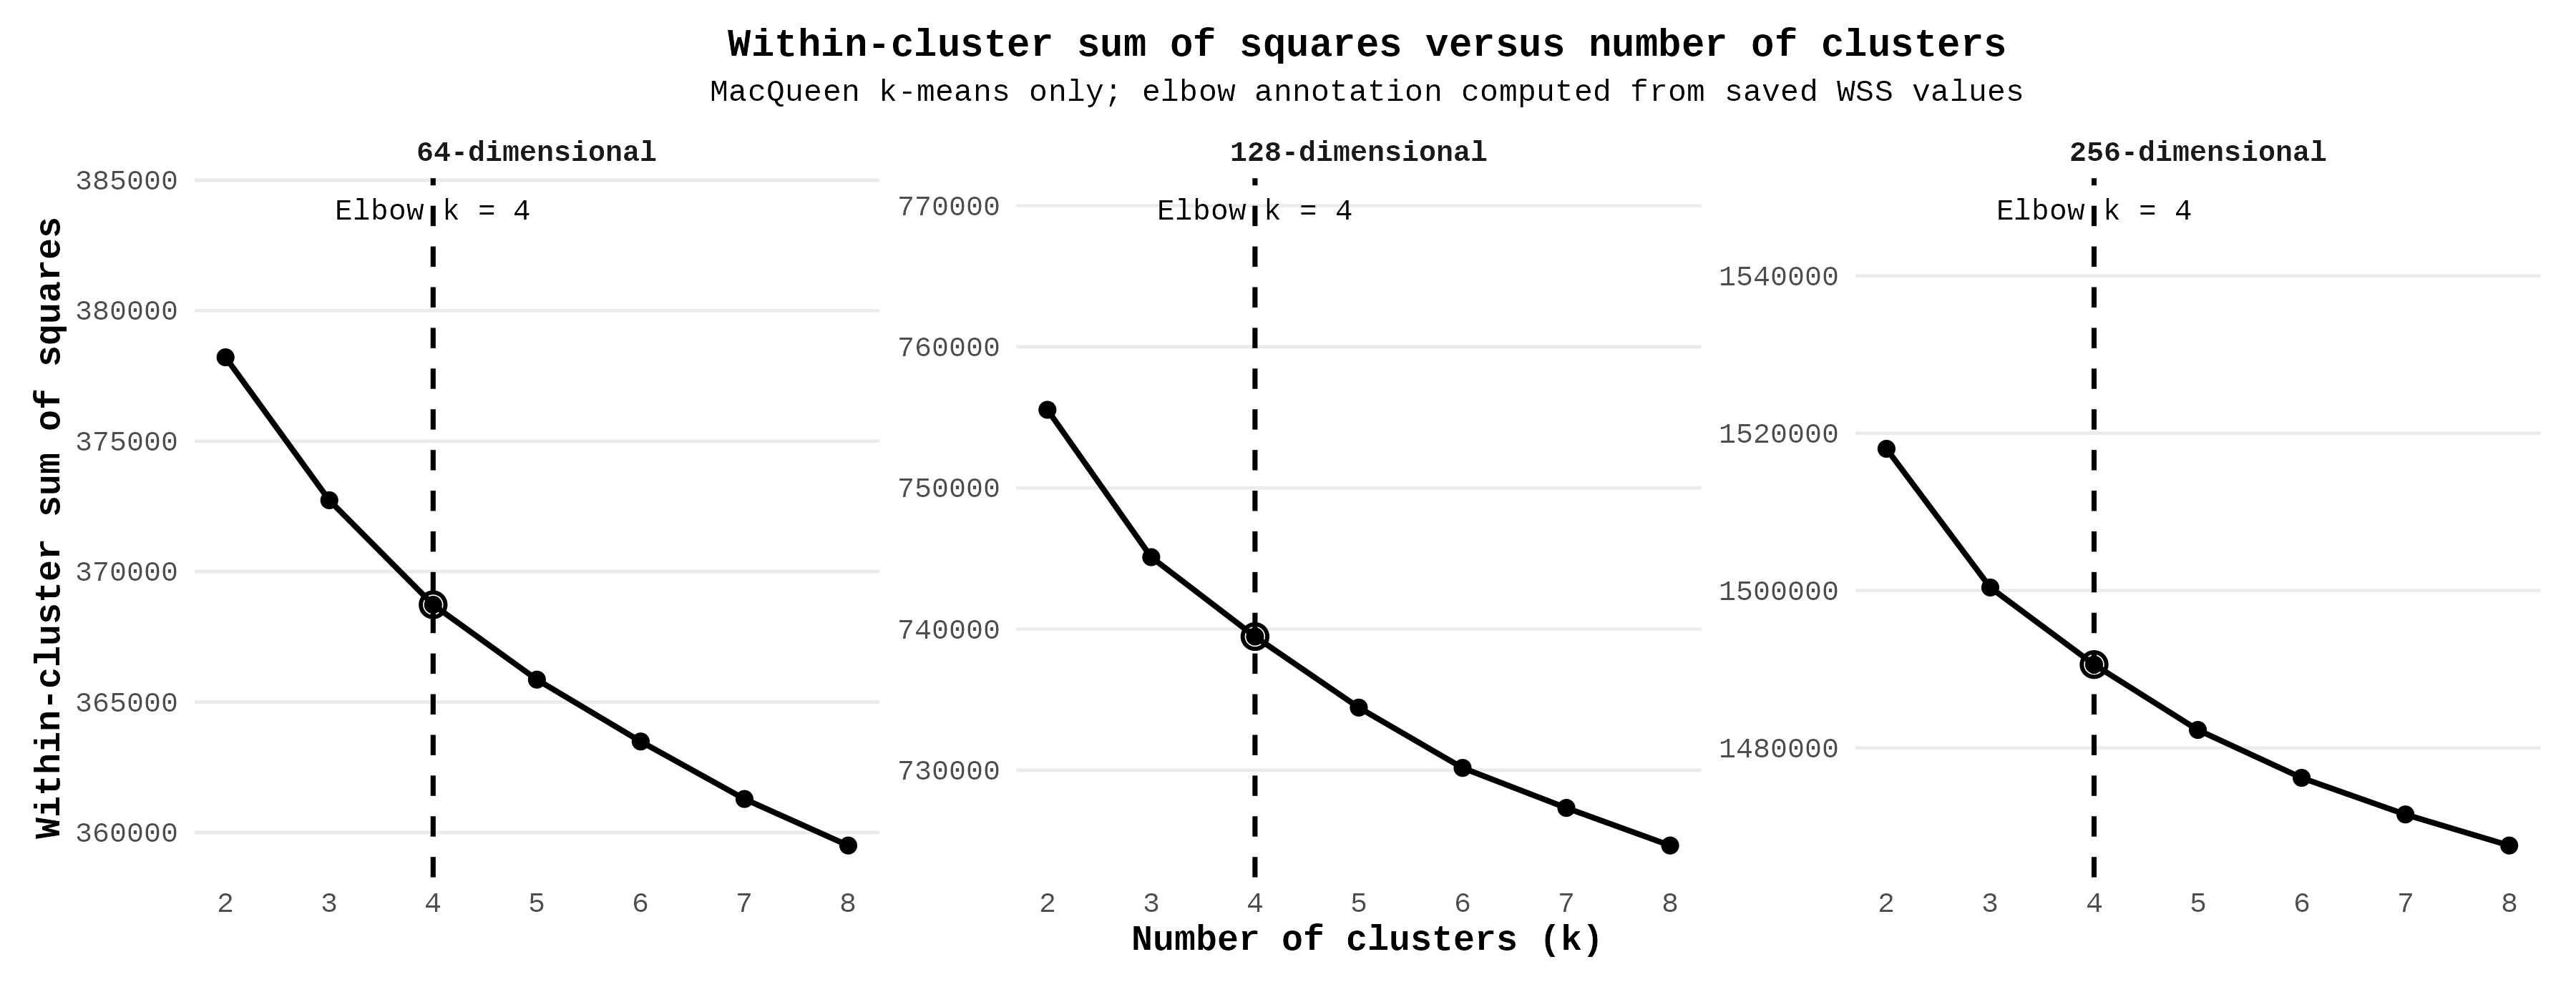
\includegraphics[width=0.85\textwidth]{figures/appendix_figureA1_kmeans_wss_vs_k_cleaned.png}
    \caption{Within-cluster sum of squares for MacQueen K-means across candidate cluster counts. The elbow diagnostic selects 4 clusters in all three embedding dimensions.}
    \label{fig-kmeans-wss-appendix}
\end{figure}

\begin{figure}[htbp]
    \centering
    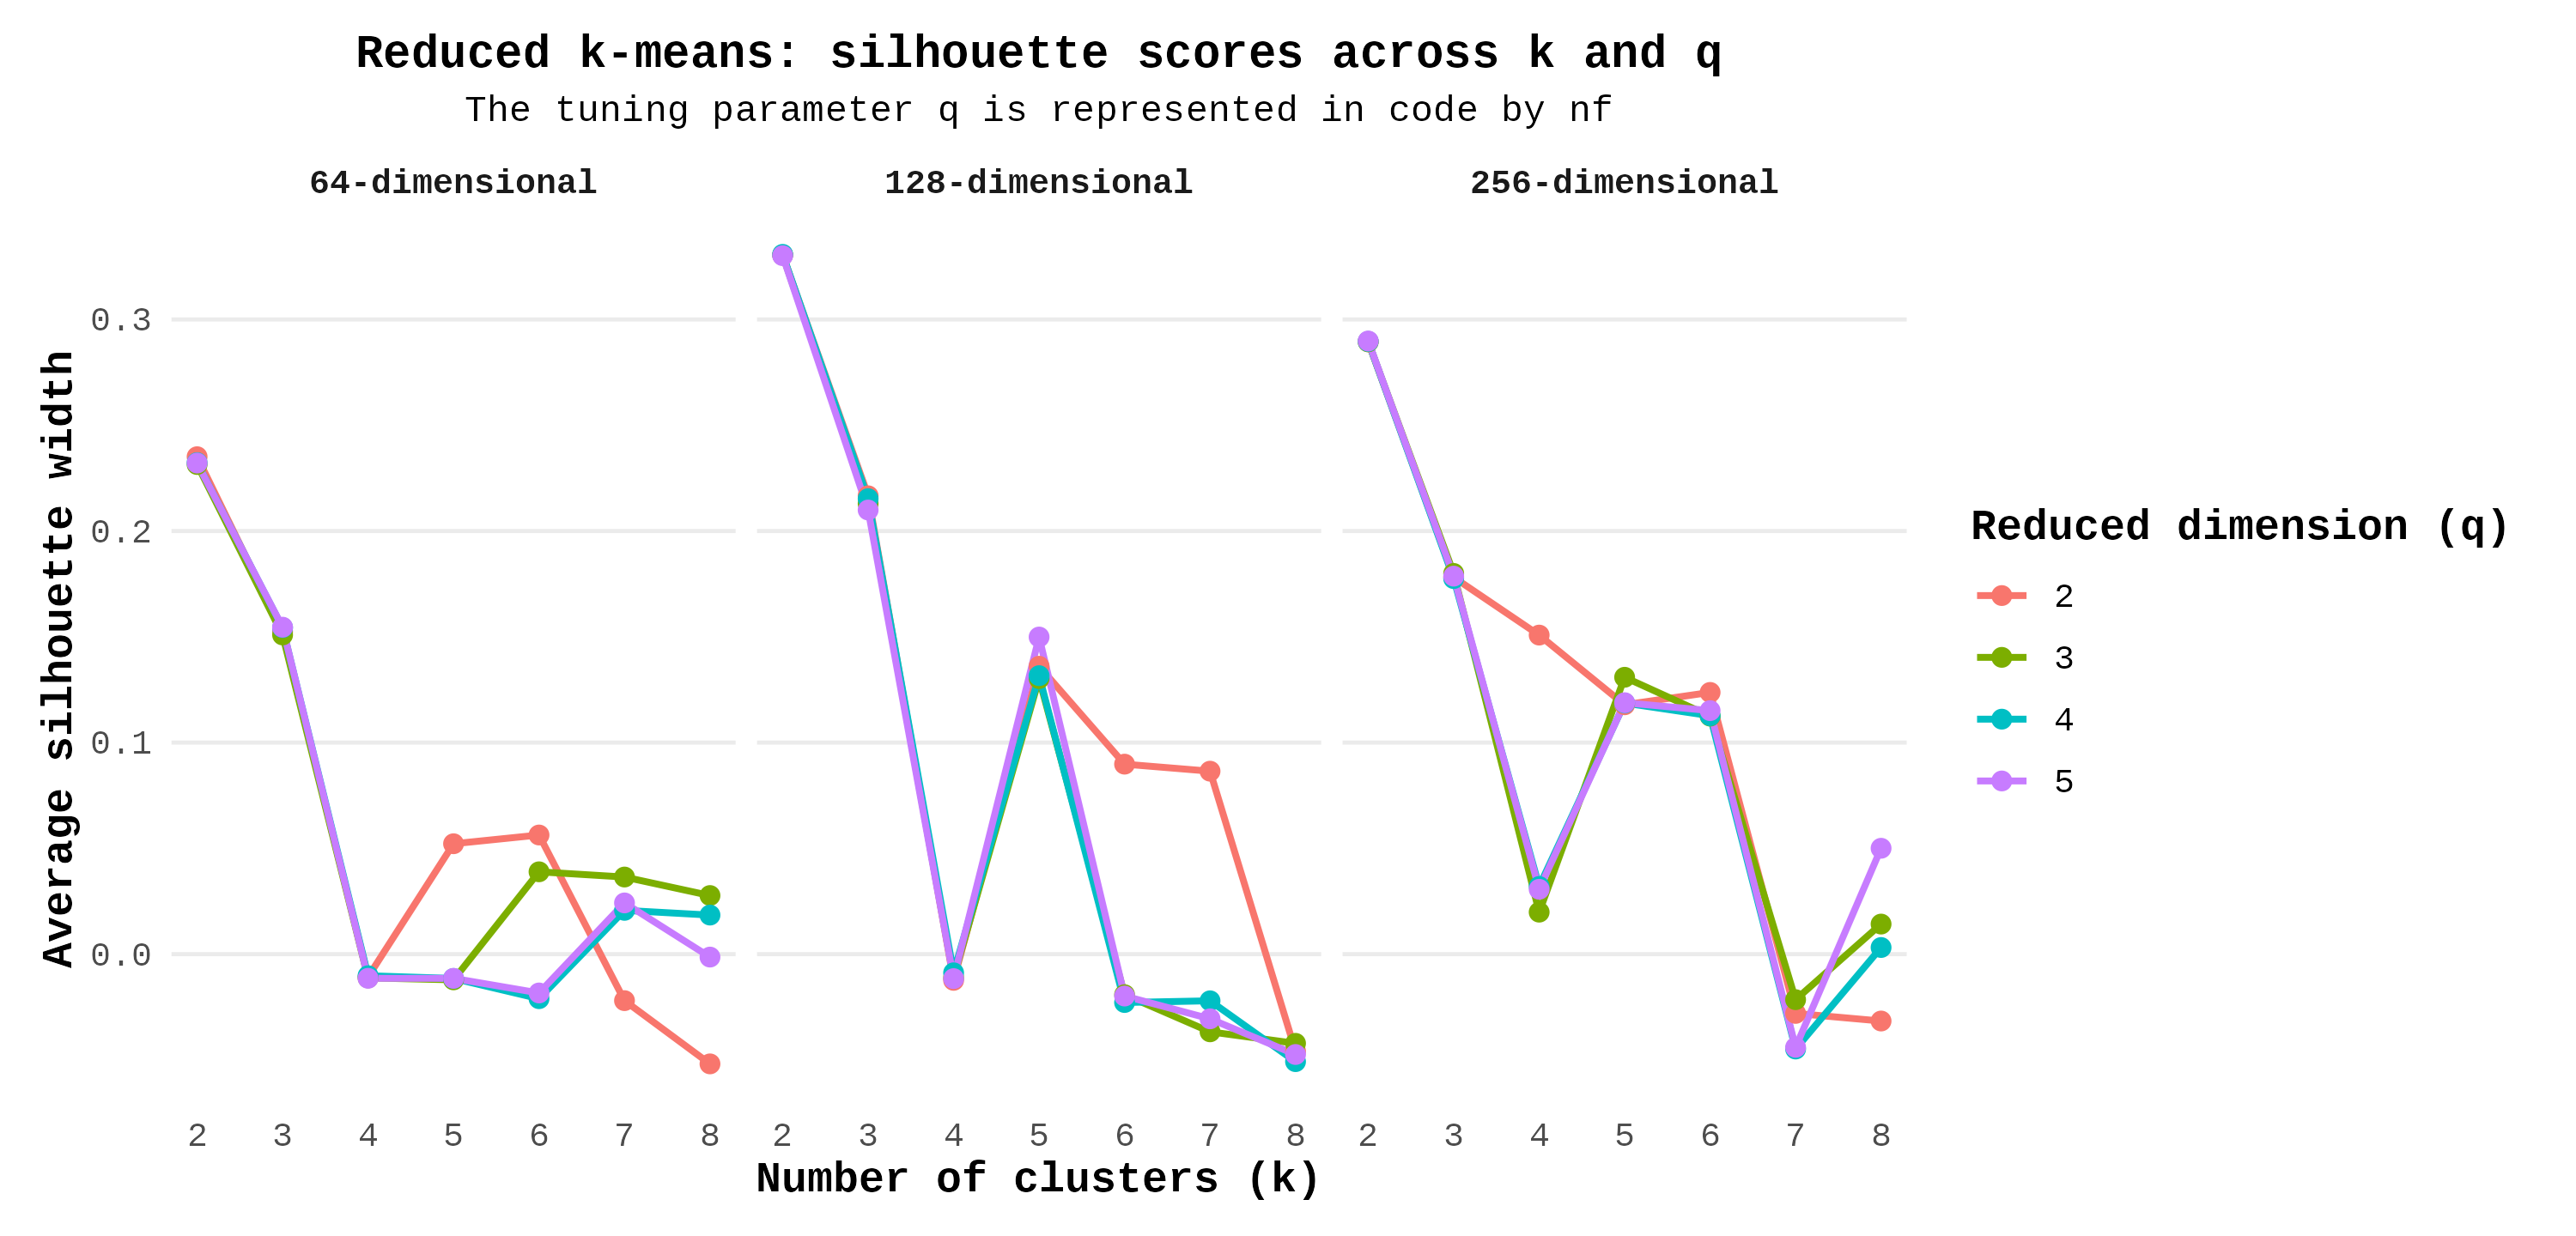
\includegraphics[width=0.85\textwidth]{figures/appendix_figureA2_rkm_silhouette_vs_k_nf.png}
    \caption{Reduced K-means silhouette values across candidate cluster counts and retained-factor settings. The strongest region lies at 3 clusters if we look at the elbow technique, and 2 clusters if we use average silhouette width alone.}
    \label{fig-rkm-grid-appendix}
\end{figure}

\begin{figure}[htbp]
    \centering
    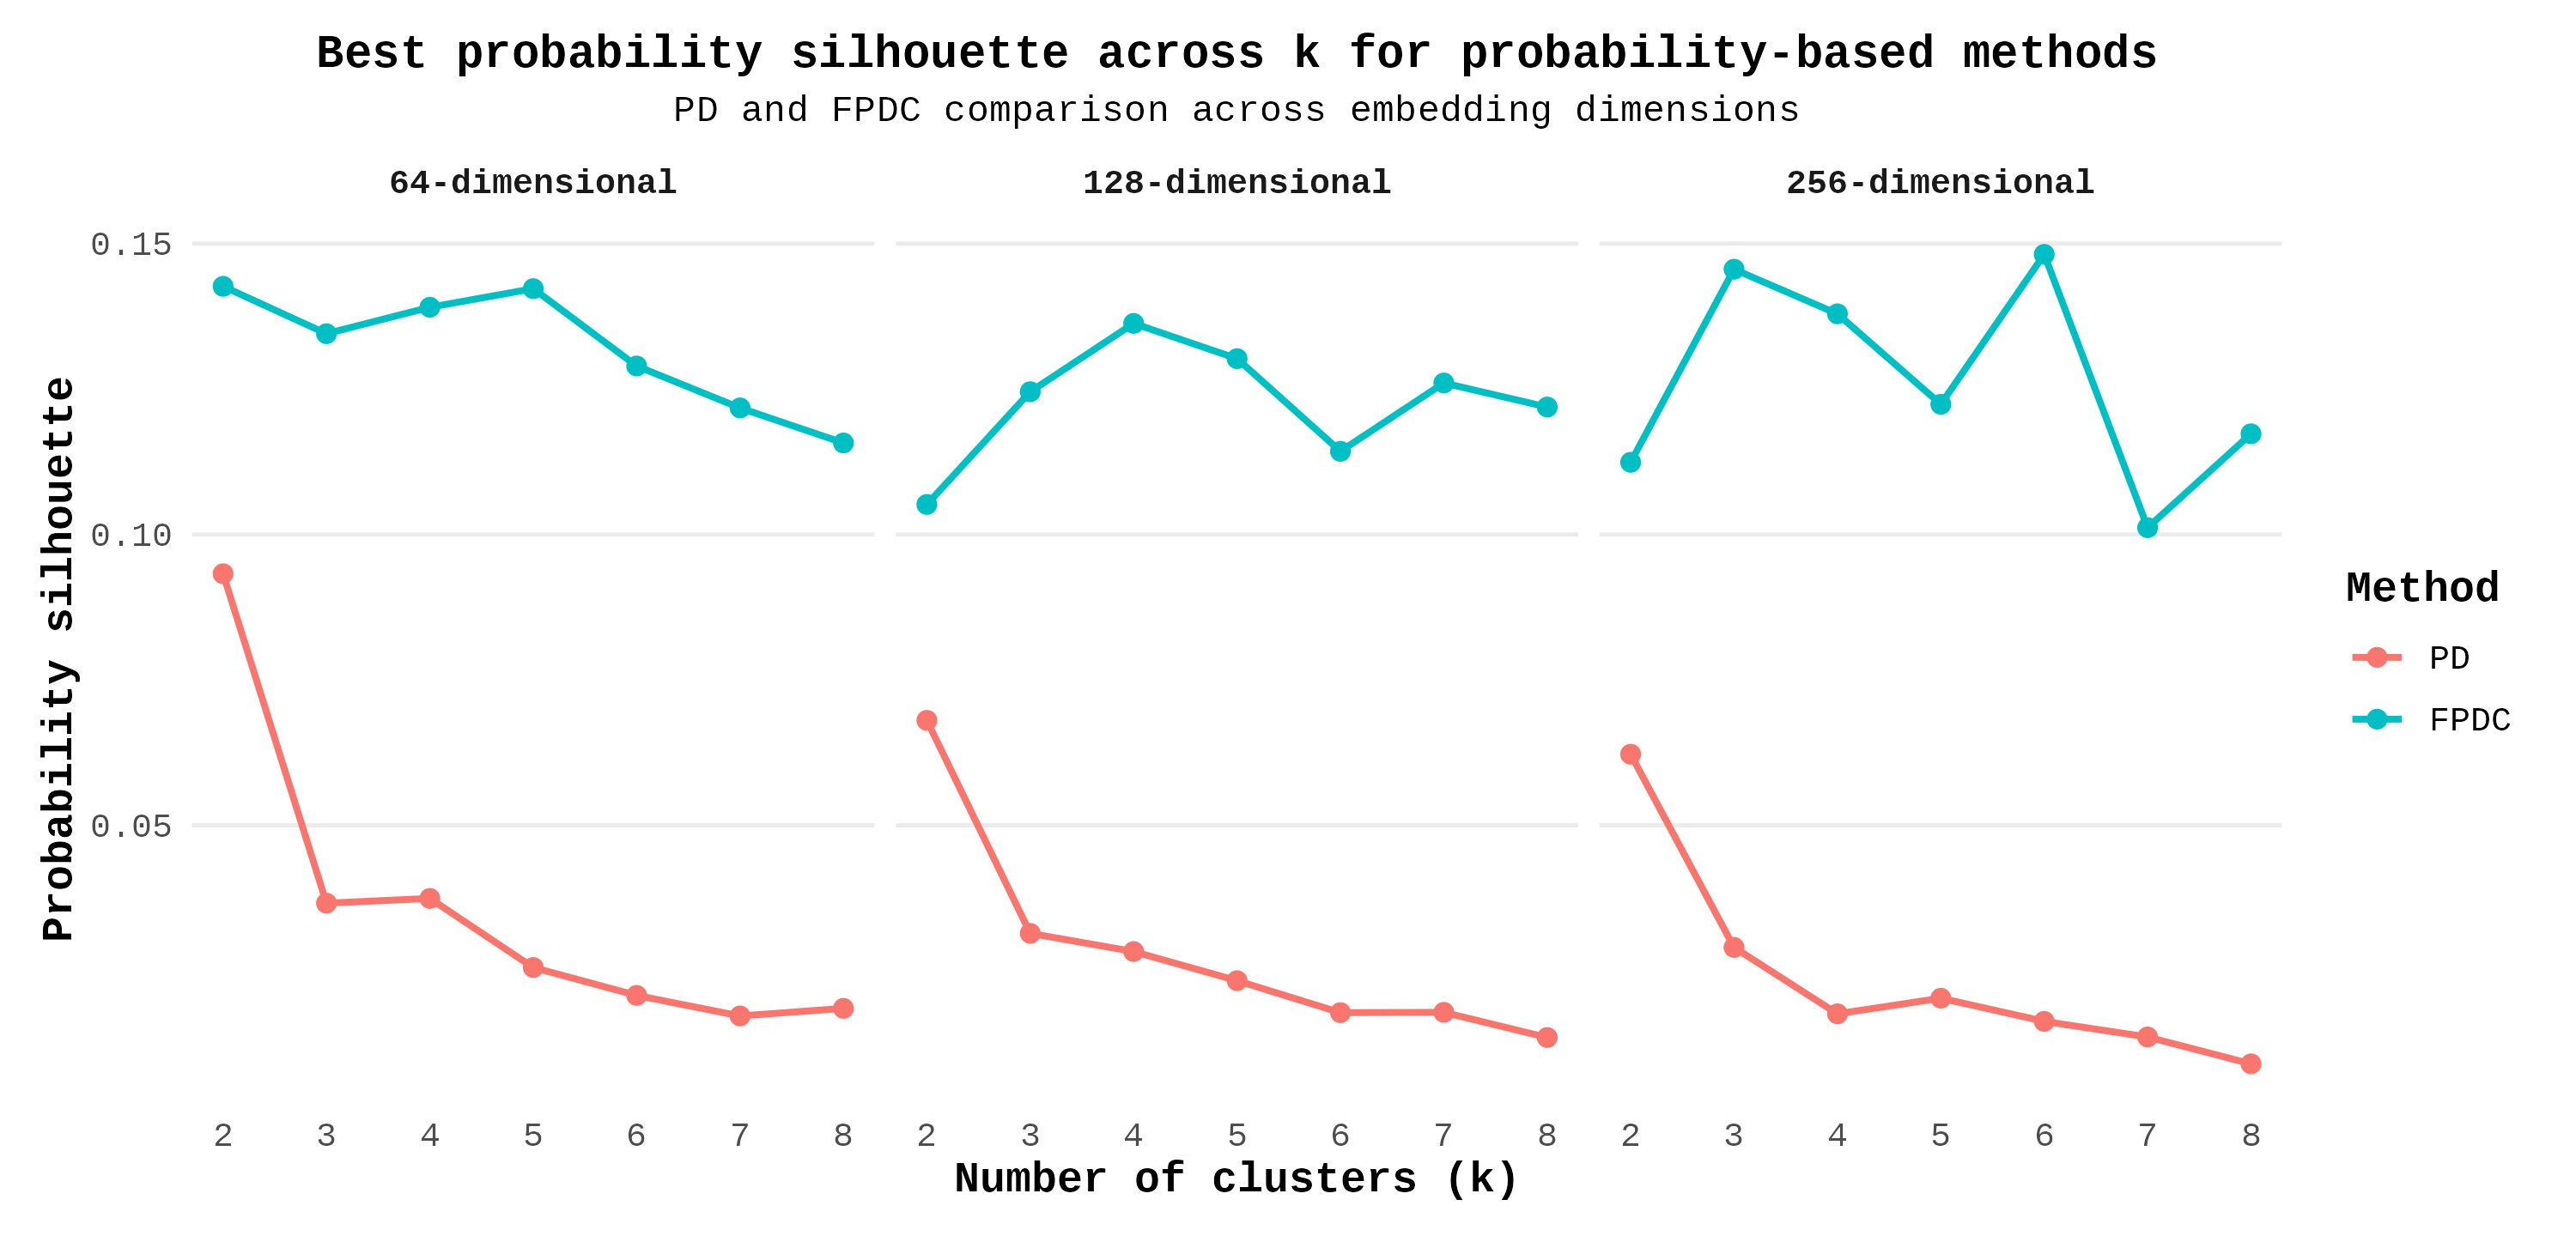
\includegraphics[width=0.85\textwidth]{figures/appendix_figureA3_probability_silhouette_pd_fpdc.png}
    \caption{Best probability silhouette across candidate cluster counts for PD clustering and FPDC. FPDC improves the soft-membership diagnostic relative to PD, but it still does not produce a strong hard partition.}
    \label{fig-prob-silhouette-appendix}
\end{figure}

\begin{figure}[htbp]
    \centering
    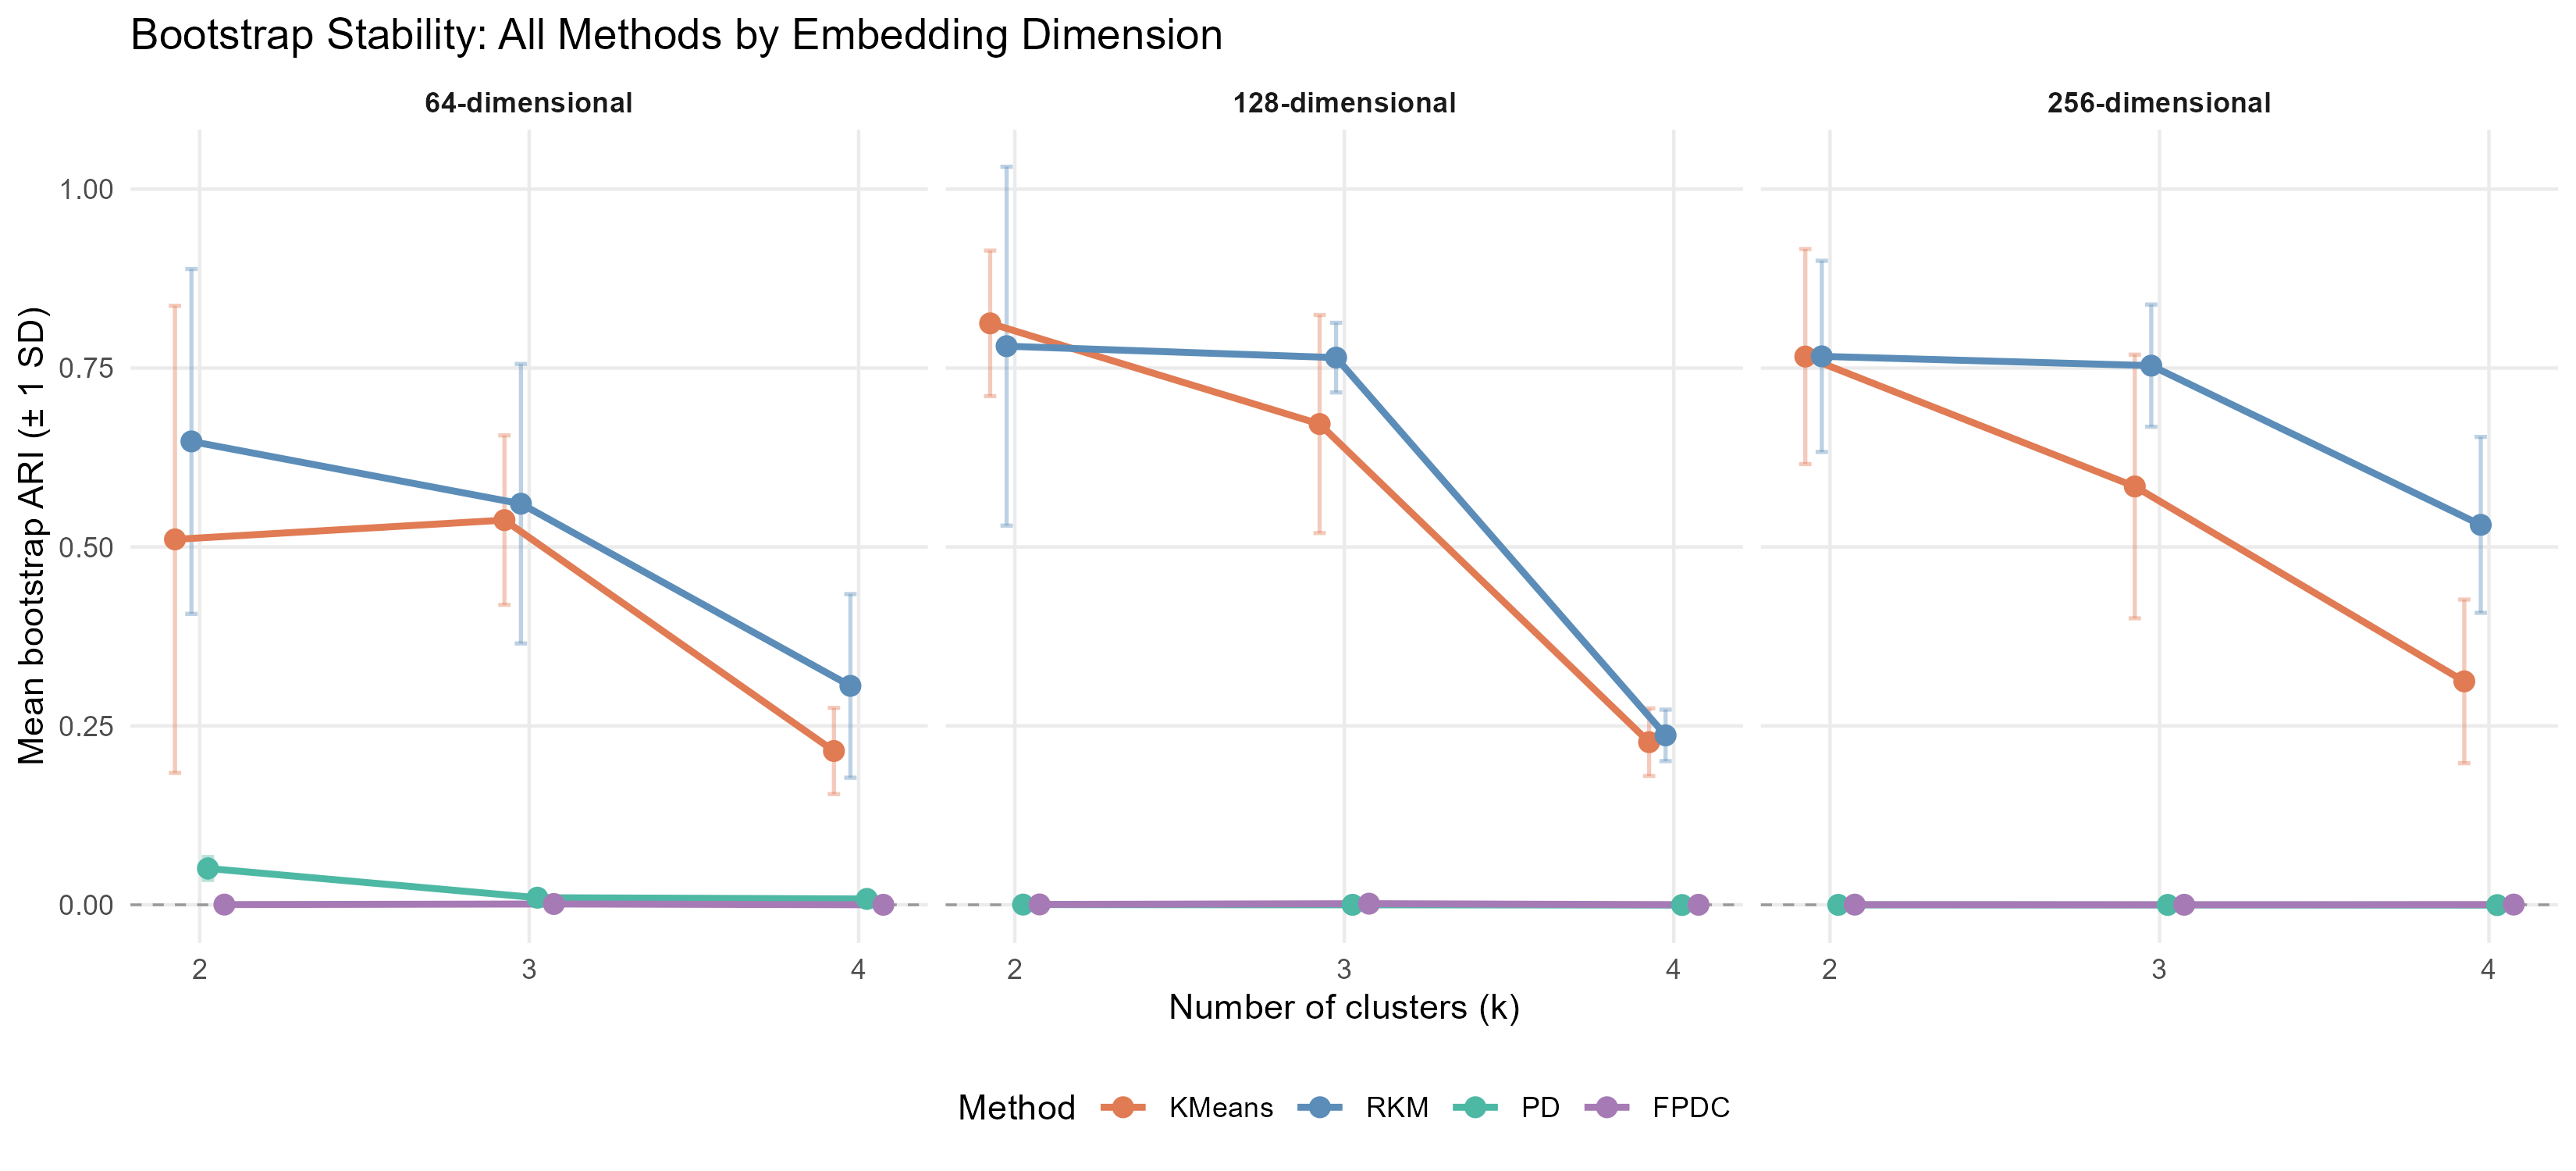
\includegraphics[width=0.85\textwidth]{figures/stability_all_methods_by_embedding.png}
    \caption{Bootstrap stability for all methods across embedding dimensions and cluster counts.}
    \label{fig-stability}
\end{figure}

\begin{figure}[htbp]
    \centering
    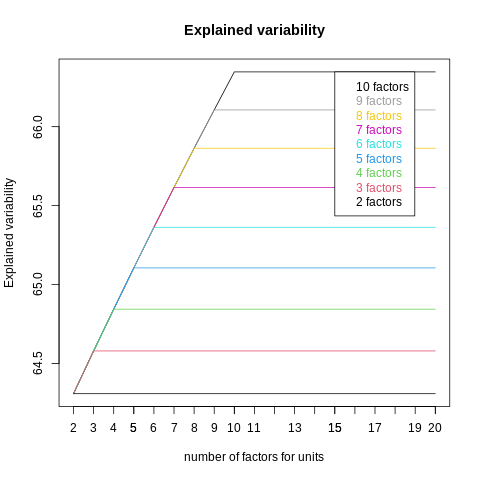
\includegraphics[width=0.45\textwidth]{figures/TuckerFactor.png}
    \caption{Tucker-factor diagnostic for the learned embeddings. The diagnostic increases smoothly as the number of retained factors grows and does not show a sharp elbow, which supports a compact retained-factor search range.}
    \label{fig-tucker-factor}
\end{figure}

\begin{table}

\caption{\label{tbl-fpdc-nu-sensitivity}FPDC sensitivity to the tuning parameter \(\nu\). Each row reports the best FPDC model within a fixed \(\nu\) value after excluding the inconsistent \(\nu=2\) pilot runs.}

\centering{

[htbp]
\centering
\small


\resizebox{\textwidth}{!}{
\begin{tabular}{rrrrrrrr}
\toprule
Embedding dimension & \(\nu\) & Clusters & Retained factors & Runtime (s) & Average Silhouette Width & Calinski--Harabasz index & Probability Silhouette \\
\midrule
64  & 6  & 2 & 4 & 241.74 & 0.012  & 70.55 & 0.143 \\
64  & 10 & 2 & 4 & 77.76  & 0.012  & 69.93 & 0.143 \\
128 & 6  & 4 & 2 & 188.16 & -0.115 & 56.43 & 0.136 \\
128 & 10 & 4 & 2 & 69.08  & -0.115 & 56.59 & 0.136 \\
256 & 6  & 3 & 2 & 170.20 & -0.056 & 63.41 & 0.146 \\
256 & 10 & 6 & 3 & 70.74  & -0.209 & 33.92 & 0.148 \\
\bottomrule
\end{tabular}
}

}

\end{table}%

\section*{References}\label{references}
\addcontentsline{toc}{section}{References}

\phantomsection\label{refs}
\begin{CSLReferences}{1}{0}
\bibitem[\citeproctext]{ref-benisrael2008pdclustering}
Ben-Israel, Adi, and Cem Iyigun. 2008. {``Probabilistic d-Clustering.''}
\emph{Journal of Classification} 25.

\bibitem[\citeproctext]{ref-desoete1994rkm}
De Soete, Geert, and J. Douglas Carroll. 1994. {``K-Means Clustering in
a Low-Dimensional {Euclidean} Space.''} In \emph{New Approaches in
Classification and Data Analysis}, edited by E. Diday, Y. Lechevallier,
M. Schader, P. Bertrand, and B. Burtschy, 212--19. Heidelberg: Springer.
\url{https://doi.org/10.1007/978-3-642-51175-2_24}.

\bibitem[\citeproctext]{ref-everitt2011cluster}
Everitt, Brian S., Sabine Landau, Morven Leese, and Daniel Stahl. 2011.
\emph{Cluster Analysis}. 5th ed. John Wiley \& Sons.

\bibitem[\citeproctext]{ref-kaufman1990finding}
Kaufman, Leonard, and Peter J. Rousseeuw. 1990. \emph{Finding Groups in
Data: An Introduction to Cluster Analysis}. John Wiley \& Sons.

\bibitem[\citeproctext]{ref-tortora2016fpdc}
Tortora, Cristina, Mireille Gettler Summa, Marina Marino, and Francesco
Palumbo. 2016. {``Factor Probabilistic Distance Clustering ({FPDC}): A
New Clustering Method for High Dimensional Data Sets.''} \emph{Advances
in Data Analysis and Classification} 10 (4): 441--64.
\url{https://doi.org/10.1007/s11634-015-0219-5}.

\bibitem[\citeproctext]{ref-tortora2024fpdclustering}
Tortora, Cristina, Nadia Vidales, Francesco Palumbo, Tanvir Kalra, and
Paul D. McNicholas. 2024. {``{FPDclustering}: A Comprehensive {R}
Package for Probabilistic Distance Clustering Based Methods.''}
\emph{Computational Statistics} 40 (2): 1123--46.
\url{https://doi.org/10.1007/s00180-024-01490-5}.

\end{CSLReferences}




\end{document}
